% chap10
\chapter{Integration of differential forms}
\label{chap:10}

Integration can be studied on many levels.
In Chap. \ref{chap:06}, the theory was developed for reasonably well-behaved functions on subintervals of the real line.
In Chap. \ref{chap:11} we shall encounter a very highly developed theory of integration that can be applied to much larger classes of functions,
whose domains are more or less arbitrary sets,
not necessarily subsets of $\R^n$.
The present chapter is devoted to those aspects of integration theory that are closely related to the
geometry of euclidean spaces, such as the change of variables formula, line integrals, and the machinery of differential forms that is used in the statement and proof of then-dimensional analogue of the fundamental theorem of calculus, namely \myKeywordred{Stokes' theorem}.

% chap10sec01

\section{Integration}
\begin{mydef}
    \label{mydef:10.1}
    Suppose $I^k$ is a $k$-cell in $\R^k$, consisting of all
    \begin{equation*}
        \mathbf{x} = (x_1,\dots,x_k)
    \end{equation*}
    such that
    \begin{equation}
        \label{eq:10.1}
        a_i \leq x_i \leq b_i
        \quad
        (i = 1,\dots, k) ,
    \end{equation}
    $I^j$ is the $j$-cell in $\R^j$ defined by the first $j$ inequalities (\ref{eq:10.1}), and f is a real continuous function on $I^k$.

    Put $f = f_k$, and define $f_{k-1}$ on $I^{k-1}$ by
    \begin{equation*}
        f_{k-1}(x_1,\dots,x_{k-1}) =
        \int_{a_k}^{b_k} f_k (x_1,\dots,x_{k-1},x_k) \d x_k .
    \end{equation*}
    The uniform continuity of $f_k$ on $I^k$ shows that $f_{k-1}$ is continuous on $I^{k-1}$.
    Hence we can repeat this process and obtain functions $f_j$, continuous on $I^j$,
    such that $f_{j-1}$ is the integral of $f_j$, with respect to $x_j$, over $[a_j, b_j]$.
    After $k$ steps we arrive at a \myKeywordblue{number} $f_0$,
    which we call the \myKeywordblue{integral of $f$ over $I^k$};
    we write it in the form
    \begin{equation}
        \label{eq:10.2}
        \int_{I^k} f(\mathbf{x}) \d \mathbf{x}
        \text{  or  }
        \int_{I^k} f.
    \end{equation}

    A priori, this definition of the integral depends on the order in which the $k$ integrations are carried out.
    However, this dependence is only apparent.
    To prove this, let us introduce the temporary notation $L(f)$ for the integral (\ref{eq:10.2}) and $L'(f)$ for the result obtained by carrying out the $k$ integrations in some other order.
\end{mydef}
\mybox{
    $L(f)$ 积分 (\ref{eq:10.2}) 暂时的记号

    $L'(f)$ 用另外的次序求这 $k$ 个积分的结果
}

\begin{thm}
    \label{thm:10.2}
    For every $f \in \mathscr{C}(I^k)$, $L(f) = L'(f)$.
\end{thm}
\mybox{对区间上的连续函数, 积分结果与积分顺序无关}
% todo add proof
\mybox{Stone-Weierstrass 定理能够用到这些函数上}

\begin{mydef}
    \label{mydef:10.3}
    The \myKeywordblue{support} of a (real or complex) function $f$ on $\R^k$ is the
    closure of the set of all points $\mathbf{x} \in R^k$
    at which $f(\mathbf{x}) \neq 0$.
    If $f$ is a continuous function with compact support,
    let $I^k$ be any $k$-cell which contains the support of $f$,
    and define
    \begin{equation}
        \label{eq:10.3}
        \int_{R^k} f =
        \int_{I^k} f .
    \end{equation}
    The integral so defined is evidently independent of the choice of $I^k$, provided only that $I^k$ contains the support of $f$.

\end{mydef}

\mybox{support 支集}

It is now tempting to extend the definition of the integral over $R^k$ to
functions which are limits (in some sense) of continuous functions with compact support.
We do not want to discuss the conditions under which this can be done;
the proper setting for this question is the Lebesgue integral.

\begin{newexample}
    \label{newexample:10.4}
    Let $Q^k$ be the $k$-simplex which consists of all points $\mathbf{x} = (x_1, \dots , x_k)$ in $\R^k$ for which $x_1 + \dots + x_k \leq 1$ and $x_i \geq 0$ for $i = 1, ... , k$.
    If $k = 3$, for example, $Q^k$ is a tetrahedron, with vertices at $\mathbf{0, e_1, e_2, e_3}$.
    If $f \in \mathscr{C}(Q^k)$,
    extend $f$ to a function on $I^k$ by setting $f(\mathbf{x}) = \mathbf{0}$ off $Q^k$, and define
    \begin{equation}
        \label{eq:10.4}
        \int_{Q^k} f =
        \int_{I^k} f .
    \end{equation}
    Here $I^k$ is the ``unit cube'' defined by
    \begin{equation*}
        0 \leq x_i \leq 1
        \quad
        (1 \leq i \leq k).
    \end{equation*}

    Since $f$ may be discontinuous on $I^k$, the existence of the integral on the right of \eqref{eq:10.4} needs proof.
    We also wish to show that this integral is independent of the order in which the $k$ single integrations are carried out.

    To do this, suppose $0 < \delta < 1$, put
    \begin{equation}
        \label{eq:10.5}
        \phi(t) = \left\{
        \begin{array}{ll}
            1                    & (t\leq 1-\delta)      \\
            \frac{(1-t)}{\delta} & (1-\delta < t \leq 1) \\
            0                    & (1<t),                \\
        \end{array}
        \right.
    \end{equation}
    and define
    \begin{equation}
        \label{eq:10.6}
        F(\mathbf{x}) =
        \phi(x_1+\cdots+x_k) f(\mathbf{x})
        \quad
        (\mathbf{x} \in I^k).
    \end{equation}
    Then $F \in \mathscr{C}(I^k)$.

    Put $\mathbf{y} = (x_1, \dots , x_{k-1})$, $\mathbf{x} = (\mathbf{y}, x_k)$.
    For each $\mathbf{y} \in I^{k-1}$, the set of all $x_k$ such that $F(\mathbf{y}, x_k) \neq f(\mathbf{y}; x_k)$ is either empty or is a segment whose length does not exceed $\delta$.
    Since $0 \leq \phi \leq 1$, it follows that
    \begin{equation}
        \label{eq:10.7}
        \left| F_{k-1}(\mathbf{y})-f_{k-1}(\mathbf{y}) \right| \leq \delta \left\| f \right\|
        \quad
        (\mathbf{y} \in I^{k-1}),
    \end{equation}
    where $\left\| f \right\|$ has the same meaning as in the proof of Theorem \ref{thm:10.2},
    and $F_{k-1}$, $f_{k-1}$ are as in Definition \ref{mydef:10.1}.

    As $\delta \rightarrow 0$, \eqref{eq:10.7} exhibits $f_{k-1}$ as a uniform limit of a sequence of continuous functions.
    Thus $f \in \mathscr{C}(I^{k-1})$, and the further integrations present no problem.

    This proves the existence of the integral \eqref{eq:10.4}.
    Moreover, \eqref{eq:10.7} shows that
    \begin{equation}
        \label{eq:10.8}
        \left|
        \int_{I^k} F(\mathbf{x}) \d \mathbf{x} -
        \int_{I^k} f(\mathbf{x}) \d \mathbf{x}
        \right| \leq
        \delta \left\| f \right\| .
    \end{equation}
    Note that \eqref{eq:10.8} is true, regardless of the order in which the $k$ single integrations are carried out.
    Since $F \in \mathscr{C}(I^k)$, $\int F$ is unaffected by any change in this order.
    Hence \eqref{eq:10.8} shows that the same is true of $\int f$

    This completes the proof.

    Our next goal is the change of variables formula stated in Theorem \ref{thm:10.9}.
    To facilitate its proof, we first discuss so-called primitive mappings, and partitions of unity.
    Primitive mappings will enable us to get a clearer picture of the local action of $\mathscr{C}'$-mapping with invertible derivative,
    and partitions of unity are a very useful device that makes it possible to use local information in a global setting.
\end{newexample}


% chap10sec02

\section{Primitive mappings}

\mybox{本原映射}

\begin{mydef}
    \label{mydef:10.5}
    If $\mathbf{G}$ maps an open set $E \subset \R^n$ into $\R^n$,
    and if there is an integer $m$ and a real function $g$ with domain $E$ such that
    \begin{equation}
        \label{eq:10.9}
        \mathbf{G(x)} = \sum_{i \neq m} x_i \mathbf{e}_i + g(\mathbf{x}) \mathbf{e}_m
        \quad
        (\mathbf{x} \in E) ,
    \end{equation}
    then we call $\mathbf{G}$ \myKeywordblue{primitive}.
    A primitive mapping is thus one that changes at most one coordinate.
    Note that (\ref{eq:10.9}) can also be written in the form
    \begin{equation}
        \label{eq:10.10}
        \mathbf{G(x)} = \mathbf{x} + \left[ g(\mathbf{x}) - x_m \right] \mathbf{e}_m .
    \end{equation}

    If $g$ is differentiable at some point $\mathbf{a} \in E$, so is $\mathbf{G}$.
    The matrix $[\alpha_{ij}]$ of the operator $\mathbf{G'(a)}$ has
    \begin{equation}
        \label{eq:10.11}
        (D_1 g)(\mathbf{a}),...
        (D_m g)(\mathbf{a}),...
        (D_n g)(\mathbf{a})
    \end{equation}
    as ots $m$th row.
    For $j \neq m$, we have $\alpha_{jj} = 1$ and $\alpha_{ij} = 0$ if $i \neq j$.
    The Jacobian of $\mathbf{G}$ at $\mathbf{a}$ is thus given by
    \begin{equation}
        \label{eq:10.12}
        J_{\mathbf{G}}(\mathbf{a}) =
        \det [\mathbf{G'(a)}] =
        (D_m g)(\mathbf{a}),
    \end{equation}
    and we see (by Theorem \ref{thm:9.36}) that $\mathbf{G'(a)}$ is
    \myKeywordblue{invertible if and only if} $(D_m g)(\mathbf{a}) \neq 0$.
\end{mydef}

\begin{mydef}
    \label{mydef:10.6}
    A linear operator $B$ on $\R^n$ that interchanges some pair of members of the standard basis and leaves the others fixed will be called a \myKeywordblue{flip}.

    For example, the flip $B$ on $\R^4$ that interchanges $e_2$ and $e_4$ has the form
    \begin{equation}
        \label{eq:10.13}
        B(x_1 \mathbf{e}_1 +
        x_2 \mathbf{e}_2 +
        x_3 \mathbf{e}_3 +
        x_4 \mathbf{e}_4) =
        x_1 \mathbf{e}_1 +
        x_2 \mathbf{e}_4 +
        x_3 \mathbf{e}_3 +
        x_4 \mathbf{e}_2
    \end{equation}
    or, equivalently,
    \begin{equation}
        \label{eq:10.14}
        B(x_1 \mathbf{e}_1 +
        x_2 \mathbf{e}_2 +
        x_3 \mathbf{e}_3 +
        x_4 \mathbf{e}_4) =
        x_1 \mathbf{e}_1 +
        x_4 \mathbf{e}_2 +
        x_3 \mathbf{e}_3 +
        x_2 \mathbf{e}_4 .
    \end{equation}
    Hence $B$ can also be thought of as interchanging two of the coordinates,
    rather that two basis vectors.

    In the proof that follows, we shall use the projections $P_0,\dots,P_n$ in $\R^n$, defined by $P_0 \mathbf{x = 0}$ and
    \begin{equation}
        \label{eq:10.15}
        P_m \mathbf{x} =
        x_1 \mathbf{e}_1 + \dots
        x_m \mathbf{e}_m
    \end{equation}
    for $1 \leq m \leq n$.
    Thus $P_m$ is the projection whose range and null space are spanned by $\{\mathbf{e_1,...,e_m}\}$ and $\{\mathbf{e_{m+1},...,e_n}\}$,
    respectively.
\end{mydef}

\begin{thm}
    \label{thm:10.7}
    Suppose $\mathbf{F}$ is a $\mathscr{C}'$-mapping of an open set $E \subset \R^n$ into $\R^n$, $\mathbf{0} \in E$, $\mathbf{F(0) = 0}$, and $\mathbf{F'(0)}$ is invertible.

    Then there is a neighborhood of $0$ in $\R^n$ in which a representation
    \begin{equation}
        \label{eq:10.16}
        \mathbf{F(x)} = B_1 \cdots B_{n-1} \mathbf{G_n \circ \cdots \circ G_1(x)}
    \end{equation}
    is valid.

    In (\ref{eq:10.16}), each $\mathbf{G}_i$ is a primitive $\mathscr{C}'$-mapping in some neighborhood of $\mathbf{0}$;
    $\mathbf{G}_i(\mathbf{0})=\mathbf{0}$, $\mathbf{G}'_i(\mathbf{0})$ is invertible, and each $B_i$ is either a flip or the identity operator.
\end{thm}

Briefly, (\ref{eq:10.16}) represents $\mathbf{F}$ locally as a composition of primitive mappings and flips

% todo add proof



% chap10sec03

\section{Partitions of unity}

\begin{thm}
    \label{thm:10.8}
    Suppose $K$ is a compact subset of $\R^n$,
    and $\{V_{\alpha}\}$ is an open cover of $K$.
    Then there exist functions $\psi_1, \dots, \psi_s \in \mathscr{C}(\R^n)$
    such that
    \begin{enumerate}
        \item $0 \leq \psi_i \leq 1$ for $1 \leq i \leq s$;
        \item each $\psi_i$ has its support in some $V_{\alpha}$, and
        \item $\psi_1 (\mathbf{x}) + \cdots + \psi_s(\mathbf{x}) = 1$ for every $\mathbf{x} \in K$.
    \end{enumerate}
\end{thm}

Because of (c), $\{\psi_i\}$ is called a partition of unity,
and (b) is sometimes expressed by saying that $\{\psi_i\}$ is subordinate to the cover $\{V_{\alpha}\}$.

\begin{myCorollary*}
    If $f \in \mathscr{C}(\R^n)$ and the support of $f$ lies in $K$, then
    \begin{equation}
        \label{eq:10.25}
        f = \sum_{i=1}^{s} \psi_i f .
    \end{equation}
    Each $\psi_i f$ has its support in some $V_{\alpha}$.
\end{myCorollary*}

The point of (\ref{eq:10.25}) is that it furnishes a representation of $f$ as a sum of continuous functions $\psi_i f$ with ``small'' supports.

% todo add proof


% chap10sec04
\section{Change of variables}
\mybox{变量代换}

We can now describe the effect of a change of variables on a multiple integral.
For simplicity, we confine ourselves here to continuous functions with compact
support, although this is too restrictive for many applications.
This is illustrated by Exercises \ref{ex:10.9} to \ref{ex:10.13}

\begin{thm}
    \label{thm:10.9}
    Suppose $T$ is a 1-1 $\mathscr{C}'$-mapping of an open set $E \subset \R^k$ into $\R^k$
    such that $J_T(\mathbf{x}) \neq 0$ for all $\mathbf{x} \in E$.
    If $f$ is a continuous function on $\R^k$ whose support is compact and lies in $T(E)$, then
    \begin{equation}
        \label{eq:10.31}
        \int_{\R^k} f(\mathbf{y}) \d \mathbf{y} =
        \int_{\R^k} f(T \mathbf{x}) \left| J_T(\mathbf{x}) \right| \d \mathbf{x} .
    \end{equation}
\end{thm}

% todo add words

% todo add proof


% chap10sec05
\section{Differential forms}

We shall now develop some of the machinery that is needed for the $n$-dimensional version of the fundamental theorem of calculus which is usually called \myKeywordblue{Stokes' theorem}.
The original form of Stokes' theorem arose in applications of
vector analysis to electromagnetism and was stated in terms of the curl of a
vector field.
Green's theorem and the divergence theorem are other special cases.
These topics are briefly discussed at the end of the chapter.
\mybox{斯托克斯定理}

It is a curious feature of Stokes' theorem that the only thing that is difficult
about it is the elaborate structure of definitions that are needed for its statement.
These definitions concern differential forms, their derivatives, boundaries, and
orientation. Once these concepts are understood, the statement of the theorem
is very brief and succinct, and its proof presents little difficulty.

Up to now we have considered derivatives of functions of several variables
only for functions defined in open sets. This was done to avoid difficulties that
can occur at boundary points. It will now be convenient, however, to discuss
differentiable functions on \myKeywordblue{compact} sets. We therefore adopt the following
convention:

To say that $\mathbf{f}$ is a $\mathscr{C}'$-mapping (or a $\mathscr{C}''$-mapping) of a compact set
$D \subset \R^k$ into $\R^n$ means that there is a $\mathscr{C}'$-mapping (or a $\mathscr{C}''$-mapping) $\mathbf{g}$ of
an open set $W \subset \R^k$ into $\R^n$ such that $D \subset W$ and such that $\mathbf{g(x) = f(x)}$ for all $\mathbf{x} \in D$.

\begin{mydef}
    \label{mydef:10.10}
    Suppose $E$ is an open set in $\R^n$.
    A $k$-surface in E is a $\mathscr{C}'$-mapping $\Phi$ from a compact set $D \subset \R^k$ into $E$.

    $D$ is called the \myKeywordblue{parameter domain} of $\Phi$.
    Points of $D$ will be denoted by $\mathbf{u} = (u_1, \dots , u_k)$.
\end{mydef}

We shall confine ourselves to the simple situation in which $D$ is either a $k$-cell or the $k$-simplex $Q^k$ described in Example 10.4. The reason for this is that we shall have to integrate over $D$,
and we have not yet discussed integration over more complicated subsets of $\R^k$.
It will be seen that this restriction on $D$
(which will be tacitly made from now on) entails no significant loss of generality in the resulting theory of differential forms.

We stress that $k$-surfaces in $E$ are defined to be \myKeywordblue{mappings} into $E$, not subsets of $E$.
This agrees with our earlier definition of curves (Definition \ref{mydef:6.26}).
In fact, $1$-surfaces are precisely the same as continuously differentiable curves.

\begin{mydef}
    \label{mydef:10.11}
    Suppose $E$ is an open set in $\R^n$.
    A \myKeywordblue{differential form of order} $k \geq 1$ in $E$
    (briefly, a $k$-form in $E$) is a function $\omega$,
    symbolically represented by the sum
    \begin{equation}
        \label{eq:10.34}
        \omega - \sum a_{i_1 \cdots i_k} (\mathbf{x})
        \d x_{i_1} \wedge \cdots \wedge
        \d x_{i_k}
    \end{equation}
    (the indices $i_1 , ... , i_k$ range independently from 1 to $n$), which assigns to each $k$-surface $\Phi$ in $E$ a number $\omega(\Phi) = \int_{\Phi} \omega$,
    according to the rule
    \begin{equation}
        \label{eq:10.35}
        \int_{\Phi} \omega =
        \int_{D} \sum a_{i_1 \cdots i_k} (\mathbf{\Phi(u)}) \frac{\partial (x_{i_1},...,x_{i_k})}{\partial (u_{1},...,u_{k})} \d \mathbf{u} ,
    \end{equation}
    where $D$ is the parameter domain of $\Phi$.

    The functions $a_{i_1 \dots i_k}$ are assumed to be real and continuous in $E$.
    If $\phi_1 , ... , \phi_n$ are the components of $\Phi$, the Jacobian in (\ref{eq:10.35}) is the one determined by the mapping
    \begin{equation*}
        (u_1,..,u_k) \rightarrow
        (\phi_{i_1}(\mathbf{u}),..,\phi_{i_k}(\mathbf{u})) .
    \end{equation*}

    Note that the right side of (\ref{eq:10.35}) is an integral over $D$, as defined in Definition \ref{mydef:10.1} (or Example 10.4) and that (\ref{eq:10.35}) is the \emph{definition} of the symbol $\int_{\Phi} \omega$.

    A $k$-form $\omega$ is said to be of class $\mathscr{C}'$ or $\mathscr{C}''$
    if the functions $a_{i_1 \cdots i_k}$ in (\ref{eq:10.34}) are all of class $\mathscr{C}'$ or $\mathscr{C}''$.

    A 0-form in E is defined to be a continuous function in $E$.
\end{mydef}


\begin{newexample}
    \label{newexample:10.12}
    \begin{enumerate}[(a)]
        \item Let $\gamma$ be a 1-surface (a curve of class $\mathscr{C}$) in $\R^3$, with parameter domain $[0, 1 ]$.
              Write $(x, y, z)$ in place of $(x_1, x_2 , x_3)$, and put
              \begin{equation*}
                  \omega = x \d y + y \d x .
              \end{equation*}
              Then
              \begin{equation*}
                  \int_{\gamma} \omega = \int_{0}^{1} \left[ \gamma_1(t) \gamma'_2(t)+\gamma_2(t) \gamma'_1(t) \right] \d t =
                  \gamma_1(1)
                  \gamma_2(1) -
                  \gamma_1(0)
                  \gamma_2(0) .
              \end{equation*}
              Note that in this example $\int_{\gamma} \omega$ depends only on the initial point $\gamma(0)$ and on the end point $\gamma(1)$ of $\gamma$.
              In particular, $\int_{\gamma} \omega = 0$ for every closed curve $\gamma$.
              (As we shall see later, this is true for every $1$-form w which is \myKeywordblue{exact}.) \\
              Integrals of I-forms are often called line \myKeywordblue{integrals}.
        \item Fix $a>0,b>0$, and define
              \begin{equation*}
                  \gamma(t) = (a \cos t, b \sin t)
                  \quad
                  (0 \leq t \leq 2\pi),
              \end{equation*}
              so that $\gamma$ is closed curve in $\R^2$.
              (Its range is an ellipse.)
              Then
              \begin{equation*}
                  \int_{\gamma} x \d y =
                  \int_{0}^{2\pi} ab \cos ^2 t \d t =
                  \pi ab,
              \end{equation*}
              whereas
              \begin{equation*}
                  \int_{\gamma} y \d x =
                  -\int_{0}^{2\pi} ab \sin ^2 t \d t =
                  -\pi ab,
              \end{equation*}
              Note that $\int_{\gamma} x \d y$ is the area of the region bounded by $\gamma$.
              This is a special case of Green's theorem.
        \item Let $D$ be the 3-cell defined by
              \begin{equation*}
                  0 \leq r \leq 1,
                  \quad
                  0 \leq \theta \leq \pi,
                  \quad
                  0 \leq \phi \leq 2\pi.
              \end{equation*}
              Define $\Phi(r,\theta,\phi)=(x,y,z)$, where
              \begin{align*}
                  x & = r \sin \theta \cos \phi \\
                  y & = r \sin \theta \sin \phi \\
                  z & = r \cos \theta.
              \end{align*}
              Then
              \begin{equation*}
                  J_{\Phi}(r,\theta,\phi) =
                  \frac{\partial(x,y,z)}{\partial(r,\theta,\phi)} =
                  r^2 \sin \theta.
              \end{equation*}
              Hence
              \begin{equation}
                  \label{eq:10.36}
                  \int_{\Phi} \d x \wedge \d y \wedge \d z =
                  \int_{D} J_{\Phi} = \frac{4\pi}{3} .
              \end{equation}
              Note that $\Phi$ maps $D$ onto the closed unit ball of $\R^3$, that the mapping is 1-1 in the interior of $D$ (but certain boundary points are identified by $\Phi$), and that the integral \eqref{eq:10.36} is equal to the volume of $\Phi(D)$.
    \end{enumerate}
\end{newexample}

\begin{mydef}
    \label{mydef:10.13}
    \myKeyword{Elementary properties}
    Let $\omega$, $\omega_1$, $\omega_2$ be $k$-forms in $E$.
    We write $\omega_1 = \omega_2$
    if and only if $\omega_1(\Phi) = \omega_2(\Phi)$
    for every $k$-surface $\Phi$ in $E$.
    If $c$ is a real number,
    then $c\omega$ is the $k$-form defined by
    \begin{equation}
        \label{eq:10.37}
        \int_{\Phi} c\omega =
        c\int_{\Phi} \omega ,
    \end{equation}
    and $\omega = \omega_1 + \omega_2$ means that
    \begin{equation}
        \label{eq:10.38}
        \int_{\Phi} \omega =
        \int_{\Phi} \omega_1 +
        \int_{\Phi} \omega_2
    \end{equation}
    for every $k$-surface $\Phi$ in $E$.
    As a special case of (\ref{eq:10.37}),
    note that $-\omega$ is defined so that
    \begin{equation}
        \label{eq:10.39}
        \int_{\Phi} (-\omega) =
        -\int_{\Phi} \omega ,
    \end{equation}

    Consider a $k$-form
    \begin{equation}
        \label{eq:10.40}
        \omega = a(\mathbf{x})
        \d x_{i_1}
        \wedge \cdots \wedge
        \d x_{i_k}
    \end{equation}
    and let $\overline{\omega}$ be the $k$-form obtained by interchanging some pair of subscripts in (\ref{eq:10.40})
    If (\ref{eq:10.35}) and (\ref{eq:10.39}) are combined with the fact that a determinant changes sign if two of its rows are interchanged,
    we see that
    \begin{equation}
        \label{eq:10.41}
        \overline{\omega} = -\omega.
    \end{equation}

    As a special case of this, note that the \myKeywordblue{anticommutative relation}
    \begin{equation}
        \label{eq:10.42}
        \d x_i \wedge \d x_j =
        -\d x_j \wedge \d x_i
    \end{equation}
    holds for all $i$ and $j$.
    In particular,
    \begin{equation}
        \label{eq:10.43}
        \d x_i \wedge \d x_i = 0
        \quad (i = 1, \dots, n).
    \end{equation}
    \mybox{外微分$\d x \wedge \d y$ 的性质,
        与向量外积 $\mathbf{a\times b} = -\mathbf{b\times a}$ 类似}

    More generally, let us return to (\ref{eq:10.40}),
    and assume that $i_r = i_s$ for some $r \neq s$.
    If these two subscripts are interchanged,
    then $\overline{\omega} = \omega$,
    hence $\omega = 0$, by (\ref{eq:10.41}).

    In other words, \emph{if $\omega$ is given by (\ref{eq:10.40}),
        then $\omega = 0$ unless the subscripts $i_1,\dots,i_k$ are all distinct}.

    If $\omega$ is as in (\ref{eq:10.34}), the summands with repeated subscripts can therefore be omitted without changing $\omega$.
    \mybox{
        summands means a part of sum

        部分和

        \url{https://www.dictionary.com/browse/summand}}
    \mybox{Direct Summand  直和

        Given the direct sum of additive Abelian groups $A \oplus B$,
        $A$ and $B$ are called direct summands.
        The map $i_1:A \rightarrow A \oplus B$ defined by $i(a)=a \oplus 0$ is called the injection of the first summand,
        and the map $p_1:A \oplus B \rightarrow A$ defined by $p_1(a \oplus b)=a$ is called the projection onto the first summand.
        Similar maps $i_2,p_2$ are defined for the second summand $B$. }

    It follows that 0 is the only $k$-form in any open subset of $\R^n$, if $k > n$.

    The anticommutativity expressed by (\ref{eq:10.42}) is the reason for the inordinate amount of attention that has to be paid to minus signs when studying differential forms.
\end{mydef}

\begin{mydef}
    \label{mydef:10.14}
    \myKeyword{Basic $k$-forms}
    If $i_1, \dots , i_k$ are integers such that
    $1 \leq i_1 < i_2 < \cdots < i_k \leq n$,
    and if $I$ is the ordered $k$-tuple $\{i_1, \dots , i_k\}$,
    then we call $I$ an increasing $k$-index,
    and we use the brief notation
    \begin{equation}
        \label{eq:10.44}
        \d x_I =
        \d x_{i_1} \wedge \cdots \wedge
        \d x_{i_k} .
    \end{equation}
    These forms $\d x_I$ are the so-called \myKeywordblue{basic $k$-forms in} $\R^n$.

    It is not hard to verify that there are precisely $n!/k!(n-k)!$ basic $k$-forms in $\R^k$;
    we shall make no use of this, however.

    Much more important is the fact that every $k$-form can be represented in terms of basic $k$-forms.
    To see this, note that every $k$-tuple $\{j_1 , \dots ,j_k\}$ of distinct integers can be converted to an increasing $k$-index $J$ by a finite number of interchanges of pairs;
    each of these amounts to a multiplication by $-1$, as we saw
    in Sec. \ref{eq:10.13}; hence
    \begin{equation}
        \label{eq:10.45}
        \d x_{j_1} \wedge \cdots \wedge
        \d x_{j_k} =
        \varepsilon (j_1, \dots , j_k) \d x_j
    \end{equation}
    where $\varepsilon(j_1, ... ,j_k)$ is $1$ or $-1$, depending on the number of interchanges that are needed.
    In fact, it is easy to see that
    \begin{equation}
        \label{eq:10.46}
        \varepsilon (j_1, \dots , j_k) =
        s (j_1, \dots , j_k)
    \end{equation}
    where $s$ is as in Definition \ref{mydef:9.33}.
\end{mydef}

For example,
\begin{equation*}
    \d x_1 \wedge
    \d x_5 \wedge
    \d x_3 \wedge
    \d x_2 =
    -
    \d x_1 \wedge
    \d x_2 \wedge
    \d x_3 \wedge
    \d x_5
\end{equation*}
and
\begin{equation*}
    \d x_4 \wedge
    \d x_2 \wedge
    \d x_3 =
    \d x_2 \wedge
    \d x_3 \wedge
    \d x_4 .
\end{equation*}

If every $k$-tuple in (\ref{eq:10.34}) is converted to an increasing $k$-index, then we
obtain the so-called standard presentation of $\omega$:
\begin{Beqnarray}
    \label{eq:10.47}
    \omega = \sum_{I} b_I (\mathbf{x}) \d x_I .
\end{Beqnarray}

The summation in (\ref{eq:10.47}) extends over all increasing $k$-indices $I$.
    [Of course, every increasing $k$-index arises from many (from $k!$, to be precise) $k$-tuples.
        Each $b_I$ in (\ref{eq:10.47})
        may thus be a sum of several of the coefficients that occur in (\ref{eq:10.34}).]

For example,
\begin{equation*}
    x_1 \d x_2 \wedge \d x_1 -
    x_2 \d x_3 \wedge \d x_2 +
    x_3 \d x_2 \wedge \d x_3 +
    \d x_1 \wedge \d x_2
\end{equation*}
is a 2-form in $\R^3$ whose standard presentation is
\begin{equation*}
    (1-x_1) \d x_1 \wedge \d x_2 +
    (x_2 + x_3) \d x_2 \wedge \d x_3 .
\end{equation*}

The following uniqueness theorem is one of the main reasons for the
introduction of the standard presentation of a $k$-form.

\begin{thm}
    \label{thm:10.15}
    Suppose
    \begin{equation}
        \label{eq:10.48}
        \omega = \sum_{I} b_I (\mathbf{x}) \d x_I
    \end{equation}
    is the standard presentation of a $k$-form $\omega$ in an open set $E \subset \R^n$.
    If $\omega = 0$ in $E$,
    then $b_I(\mathbf{x}) = 0$ for every increasing $k$-index $I$ and for every $\mathbf{x} \in E$.
\end{thm}

Note that the analogous statement would be false for sums such as (\ref{eq:10.34}),
since, for example,
\begin{equation*}
    \d x_1 \wedge \d x_2 +
    \d x_2 \wedge \d x_1 = 0.
\end{equation*}

% todo add proof

\begin{mydef}
    \myKeyword{Products of basic $k$-forms}
    Suppose
    \begin{equation}
        \label{eq:10.51}
        I = \{i_1,...,i_p\},
        \quad
        J = \{j_1,...,j_q\}
    \end{equation}
    where $1 \leq i_1 < \cdots < i_p \leq n$
    and $1 \leq j_1 < \cdots < j_q \leq n$ .
    The \myKeywordblue{product} of the corresponding basic forms $\d x_I$ and $\d x_J$ in $\R^n$ is a $(p + q)$ form in $\R^n$, denoted by the symbol $\d x_I \wedge \d x_J$, and defined by
    \begin{equation}
        \label{eq:10.52}
        \d x_I \wedge \d x_J =
        \d x_{i_1} \wedge \cdots \wedge
        \d x_{i_p} \wedge
        \d x_{j_1} \wedge \cdots \wedge
        \d x_{j_q}.
    \end{equation}
\end{mydef}

\begin{mydef}
    \myKeyword{Multiplication}
    Suppose $\omega$ and $\lambda$ are $p$- and $q$-forms, respectively, in
    some open set $E \subset \R^n$, with standard presentations
    \begin{equation}
        \label{eq:10.56}
        \omega = \sum_{I} b_I (\mathbf{x}) \d x_I , \quad
        \lambda = \sum_{J} c_J (\mathbf{x}) \d x_J
    \end{equation}
    where $I$ abd $J$ range over all increasing $p$-indices and over all increasing $q$-indices
    taken from the set $\{1, ... , n\}$.
\end{mydef}

\begin{mydef}
    \myKeyword{Differentiation}
    We shall now define a differentiation operator $\d$ which
    associates a $(k + 1)$-form $\d \omega$ to each $k$-form $\omega$ of class $\mathscr{C}'$ in some open set $E \in \R^n$.

    A 0-form of class $\mathscr{C}'$ in $E$ is just a real function $f \in \mathscr{C}'(E)$, and we define
    \begin{equation}
        \label{eq:10.59}
        \d f = \sum_{i=1}^{n} (D_i f) (\mathbf{x}) \d x_i .
    \end{equation}
    If $\omega = \sum b_I (\mathbf{x}) \d x_I$ is the standard presentation of a $k$-form $\omega$, and $B_I \in \mathscr{C}'(E)$ for each increasing $k$-index $I$, then we define
    \begin{equation}
        \label{eq:10.60}
        \d \omega = \sum_I (\d b_I) \wedge \d x_I .
    \end{equation}
\end{mydef}

\begin{newexample}
    Suppose $E$ is open in $\R^n$, $f \in \mathscr{C}'(E)$, and $\gamma$ is a continuously differentiable curve in $E$, with domain $[0,1]$. By (\ref{eq:10.59}) and (\ref{eq:10.35}),
    \begin{equation}
        \label{eq:10.61}
        \int_{\gamma} \d f
        = \int_{0}^{1} \sum_{i=1}^{n}
        (D_i f)(\gamma(t)) \gamma'_i (t)
        \d t .
    \end{equation}
    By the chain rule, the last integrand is $(f \circ \gamma)'(t)$.
    Hence
    \begin{equation}
        \label{eq:10.62}
        \int_{\gamma} \d f =
        f(\gamma(1)) -
        f(\gamma(0)) ,
    \end{equation}
    and we see that $\int_{\gamma} \d f$ is the same for all $\gamma$ with the same initial point and the same end point, as in (a) of Example 10.12.

    Comparison with Example 10.12(b) shows therefore that the 1-form $x \d y$ is not the derivative of any 0-form $f$.
    This could also be deduced from part (b) of the following theorem, since
    \begin{equation*}
        \d (x \d y) = \d x \wedge \d y
    \end{equation*}
\end{newexample}
\mybox{integrand 被积函数}

\begin{thm}
    \label{thm:10.20}
    \begin{asparaenum}[(a)]
        \item If $\omega$ and $\lambda$ are $k$- and $m$-forms, respectively, of class $\mathscr{C}'$ in $E$,
        then
        \begin{equation}
            \label{eq:10.63}
            \d (\omega \wedge \lambda) =
            (\d \omega) \wedge \lambda +
            (-1)^k \omega \wedge \d \lambda .
        \end{equation}
        \item If $\omega$ is of class $\mathscr{C}''$ in $E$, then $\d ^2 \omega = 0$.
    \end{asparaenum}
\end{thm}

Here $\d ^2 \omega$ means, of course, $\d (\d \omega)$.

% todo add proof

\begin{mydef}
    \myKeyword{Change of variables}
    Suppose $E$ is an open set in $\R^n$,
    $T$ is a $\mathscr{C}'$-mapping of $E$ into an open set $V \subset \R^m$,
    and $\omega$ is a $k$-form in $V$, whose standard presentation is
    \begin{equation}
        \label{eq:10.65}
        \omega = \sum_{I} b_I (\mathbf{y}) \d y_I.
    \end{equation}

    (We use $\mathbf{y}$ for points of $V$, $\mathbf{x}$ for points of $E$.)

    Let $t_1,\dots,t_m$ be the components of $T$: If
    \begin{equation*}
        \mathbf{y} = (y_1, \dots, y_m) = T(\mathbf{x})
    \end{equation*}
    then $y_i = t_i(\mathbf{x})$.
    As in (\ref{eq:10.59}),
    \begin{equation}
        \label{eq:10.66}
        \d t_i = \sum_{j=1}^{n}(D_j t_i)(\mathbf{x}) \d x_j
        \quad (1 \leq i \leq m).
    \end{equation}
    Thus each $\d t_i$ is a 1-form in $E$.

    The mapping $T$ transforms $\omega$ into a $k$-form $\omega_T$ in $E$,
    whose definition is
    \begin{equation}
        \label{eq:10.67}
        \omega_T = \sum_I b_I ((T(\mathbf{x})))
        \d t_{i_1} \wedge \cdots \wedge
        \d t_{i_k} .
    \end{equation}
    in each summand of (\ref{eq:10.67}),
    $I = \{i_1,...,i_k\}$ is an increasing $k$-index.
\end{mydef}

Our next theorem shows that addition, multiplication, and differentiation
of forms are defined in such a way that they commute with changes of variables.

\begin{thm}
    \label{thm:10.22}
    With $E$ and $T$ as in Sec. 10.21, let $\omega$ and $A$ be $k$- and $m$-forms in $V$, respectively. Then
    \begin{enumerate}[(a)]
        \item $(\omega + \lambda)_T = \omega_T + \lambda_T$ if $k = m$;
        \item $(\omega \wedge \lambda)_T = \omega_T \wedge \lambda_T$;
        \item $\d (\omega_T) = (\d \omega)_T$
              if $\omega$ is of class $\mathscr{C}'$
              and $T$ is of class $\mathscr{C}''$.
    \end{enumerate}
\end{thm}

% todo add proof

\begin{thm}
    \label{thm:10.23}
    Suppose $T$ is a $\mathscr{C}'$-mapping of an open set $E \subset \R^n$ into an open set $V \subset \R^m$,
    $S$ is a $\mathscr{C}'$-mapping of $V$ into an open set $W \subset \R^P$, and $w$ is a $k$-form in $W$,
    so that $\omega$ is a $k$-form in $V$
    and both $(\omega_S)_T$ and $\omega_{ST}$ are $k$-forms in $E$,
    where $ST$ is defined by $(ST)(\mathbf{x}) = S(T(\mathbf{x}))$.
    Then
    \begin{equation}
        \label{eq:10.71}
        (\omega_S)_T = \omega_{ST} .
    \end{equation}
\end{thm}

% todo add proof

\begin{thm}
    \label{thm:10.24}
    Suppose $\omega$ is a $k$-form in an open set $E \subset \R^n$,
    $\Phi$ is a $k$-surface in $E$, with parameter domain $D \subset \R^k$,
    and $\Delta$ is the $k$-surface in $\R^k$, with parameter domain $D$, defined by $\Delta(\mathbf{u}) = \mathbf{u}(\mathbf{u} \in D)$. Then
    \begin{equation*}
        \int_{\Phi} \omega =
        \int_{\Delta} \omega_{\Phi} .
    \end{equation*}
\end{thm}

% todo add proof

\begin{thm}
    \label{thm:10.25}
    Suppose $T$ is a $\mathscr{C}'$-mapping of an open set $E \subset \R^n$ into an open set $V \subset \R^m$,
    $\Phi$ is a $k$-surface in $E$,
    and $\omega$ is a $k$-form in $V$.

    Then
    \begin{equation*}
        \int_{T \Phi} \omega =
        \int_{\Phi} \omega_T
    \end{equation*}
\end{thm}

\begin{proof}
    Let $D$ be the parameter domain of $\Phi$ (hence also of $\Phi$) and define $\Delta$ as in Theorem \ref{thm:10.24}.

    Then
    \begin{equation*}
        \int_{T \Phi} \omega =
        \int_{\Delta} \omega_{T \Phi} =
        \int_{\Delta} (\omega_{T})_{\Phi} =
        \int_{\Phi} \omega_{T} .
    \end{equation*}

    The first of these equalities is Theorem \ref{thm:10.24}, applied to $T\Phi$ in place of $\Phi$.
    The second follows from Theorem \ref{thm:10.23}. The third is Theorem \ref{thm:10.24},
    with $\omega_T$ in place of $\omega$.
\end{proof}
% chap10sec06

\section{Simplexes and chains}

\begin{mydef}
    \label{mydef:10.26}
    \myKeyword{Affine simplexes}
    A mapping $\mathbf{f}$ that carries a vector space $X$ into a
    vector space $Y$ is said to be \emph{affine} if $\mathbf{f - f(0)}$ is linear. 
    In other words, the requirement is that
    \begin{equation}
        \label{eq:10.73}
        \mathbf{f(x)} = 
        \mathbf{f(0)} + A \mathbf{x}
    \end{equation}
    for some $A \in L(X, Y)$.

    An affine mapping of $\R^k$ into $\R^n$ is thus determined if we know $\mathbf{f}(0)$ and $\mathbf{f(e_i)}$ for $1 \leq i \leq k$; 
    as usual, $\{\mathbf{e}_1, ... , \mathbf{e}_k\}$ is the standard basis of $\R^k$.
    
    We define the \emph{standard simplex} $Q^k$ to be the set of all $\mathbf{u} \in \R^k$ of the form
    \begin{equation}
        \label{eq;10.74}
        \mathbf{u} = \sum_{i=1}^{k} \alpha_i \mathbf{e}_i
    \end{equation}
    such that $\alpha \geq 0$ for $i = 1, ... , k$ and $\sum \alpha_i \leq 1$.
    % todo
\end{mydef}

\begin{thm}
    \label{thm:10.27}
    If $\delta$ is an oriented rectilinear $k$-simplex in an open set $E \subset \R^n$ 
    and if $\overline{\Delta} = \varepsilon \delta$ then
    \begin{equation}
        \label{eq:10.81}
        \int_{\overline{\delta}} \omega = 
        \varepsilon \int_{\delta} \omega 
    \end{equation}
    for every $k$-form $\omega$ in $E$.
\end{thm}

% todo add proof

\begin{mydef}
    \label{mydef:10.28}
    \myKeyword{Affine chains}
    An \emph{affine $k$-chain} $\Gamma$ in an open set $E \subset \R^n$ is a collection of finitely many oriented affine $k$-simplexes $\delta_1, \dots, \delta_r$ in $E$. 
    These need not be distinct; 
    a simplex may thus occur in $\Gamma$ with a certain multiplicity.

    If $\Gamma$ is as above, and if $\omega$ is a $k$-form in $E$,
    we define 
    \begin{equation}
        \label{eq:10.82}
        \int_{\Gamma} \omega =
        \sum_{i=1}^{r} \int_{\sigma_i} \omega .
    \end{equation}
    % todo add word
\end{mydef}

\begin{mydef}
    \label{mydef:10.29}
    \myKeyword{Boundaires}
    For $k \geq 1$, the \emph{boundary} of the oriented affine $k$-simplex
    \begin{equation*}
        \delta = \left[ \mathbf{p_0,p_1,\dots,p_k} \right]
    \end{equation*}
    is defined to be the affine $(k - 1)$-chain
    \begin{equation}
        \label{eq:10.85}
        \partial \delta = \sum_{j=0}^{k} (-1)^j
        \left[ \mathbf{p_0,p_1,\dots,p_{j-1},p_{j+1},\dots,p_k} \right]
    \end{equation}
\end{mydef}

For example, if $\sigma = [\mathbf{p}_0 , \mathbf{p}_1, \mathbf{p}_2 ]$, then
\begin{equation*}
    \partial\sigma = 
    [\mathbf{p}_1, \mathbf{p}_2] - 
    [\mathbf{p}_0, \mathbf{p}_2] + 
    [\mathbf{p}_0, \mathbf{p}_1] = 
    [\mathbf{p}_0, \mathbf{p}_1] + 
    [\mathbf{p}_1, \mathbf{p}_2] + 
    [\mathbf{p}_2, \mathbf{p}_0] ,
\end{equation*}
which coincides with the usual notion of the oriented boundary of a triangle.
For $1 \leq j \leq k$, observe that the simplex $\sigma_j = [\mathbf{p}_0 , ... , \mathbf{p}_{i- 1} , \mathbf{p}_{i+ 1}, ... , \mathbf{p}_k]$
which occurs in \eqref{eq:10.85} has $Q^{k- 1}$ as its parameter domain and that it is defined by
\begin{equation}
    \label{eq:10.86}
    \sigma_j(\mathbf{u}) = \mathbf{p}_0 + B\mathbf{u} 
    \quad 
    (\mathbf{u} \in Q^{k-1}),
\end{equation}
where $B$ is the linear mapping from $\R^{k-1}$ to $\R^n$ determined by 
\begin{align*}
    B\mathbf{e}_i &= \mathbf{p}_i - \mathbf{p}_0 \quad (\text{if } 1 \leq i \leq j-1) , \\
    B\mathbf{e}_i &= \mathbf{p}_{i+1} - \mathbf{p}_0 \quad (\text{if } j \leq i \leq k-1) .
\end{align*}

The simplex 
\begin{equation*}
    \sigma_0 = [\mathbf{p}_1,\mathbf{p}_2,\dots,\mathbf{p}_k]
\end{equation*}
which also occurs in \eqref{eq:10.85}, is given by the mapping
\begin{equation*}
    \sigma_0(\mathbf{u}) = \mathbf{p}_1 + B \mathbf{u},
\end{equation*}
where $B\mathbf{e}_i = \mathbf{p}_{i+1} - \mathbf{p}_1$ for $1 \leq i \leq k-1$.



\begin{mydef}
    \label{mydef:10.30}
    \myKeyword{Differentiable simplexes and chains}
    Let $T$ be a $\mathscr{C}''$-mapping of an open set $E \subset \R^n$ into an open set $V \subset \R^m$; 
    $T$ need not be one-to-one. 
    If $\sigma$ is an oriented affine $k$-simplex in $E$, then the composite mapping $\Phi = T \circ \sigma$
    (which we shall sometimes write in the simpler form $T\sigma$) 
    is a $k$-surface in $V$, with parameter domain $Q^k$. 
    We call $\Phi$ an \myKeywordblue{oriented $k$-simplex of class $\mathscr{C}''$}.

    A finite collection $\Psi$ of oriented $k$-simplexes $\Phi_1, ... , \Phi_r$ of class $\mathscr{C}''$ in $V$
    is called a \myKeywordblue{$k$-chain of class $\mathscr{C}''$} in $V$. 
    If $\omega$ is a $k$-form in $V$, we define
    \begin{equation}
        \label{eq:10.87}
        \int_{\Psi} \omega = 
        \sum_{i=1}^{r} \int_{\Phi i} \omega
    \end{equation}
    and use the corresponding notation $\Psi = \sum \Phi_i$.

    If $\Gamma = \sum \sigma_i$ is an affine chain 
    and if $\Phi_i = T \circ \sigma_i$, 
    we also write $\Psi = T \circ \Gamma$, 
    or 
    \begin{equation}
        \label{eq:10.88}
        T\left( \sum \sigma_i \right) = \sum T \sigma_i .
    \end{equation}
    The boundary $\partial \Phi$ of the oriented $k$-simplex $\Phi = T \circ \sigma$ a is defined to be the $(k - 1)$ chain
    \begin{equation}
        \label{eq:10.89}
        \partial \Phi = T \left( \partial \sigma \right) .
    \end{equation}

    In justification of \eqref{eq:10.89}, observe that if $T$ is affine, 
    then $\Phi = T \circ \sigma$ is an oriented affine $k$-simplex, 
    in which case \eqref{eq:10.89} is not a matter of definition, 
    but is seen to be a consequence of \eqref{eq:10.85}. 
    Thus \eqref{eq:10.89} generalizes this special case.

    It is immediate that $\partial \Phi$ is of class $\mathscr{C}''$ if this is true of $\Phi$.

    Finally, we define the boundary $\partial \Phi$ of the $k$-chain $\Psi = \sum \Phi_i$ to be the $(k - 1)$ chain
    \begin{equation}
        \label{eq:10.90}
        \partial \Psi = \sum \partial \Phi_i ,
    \end{equation}
\end{mydef}

\begin{mydef}
    \label{mydef:10.31}
    \myKeyword{Positively oriented boundaries}
    So far we have associated boundaries to chains, not to subsets of $\R^n$. 
    This notion of boundary is exactly the one that is most suitable for the statement and proof of Stokes' theorem.
    However, in applications, especially in $\R^2$ or $\R^3$, it is customary and convenient to talk about ``oriented boundaries'' of certain sets as well. 
    We shall now describe this briefly. 
    
    Let $Q^n$ be the standard simplex in $\R^n$, 
    let $\sigma_0$ be the identity mapping with domain $Q^n$. 
    As we saw in Sec. \ref{mydef:10.26}, $\sigma_0$ may be regarded as a positively oriented n-simplex in $\R^n$. 
    Its boundary $\partial\sigma_0$ is an affine $(n - 1)$-chain. 
    This chain is called the positively oriented boundary of the set $Q^n$. 
    
    For example, the positively oriented boundary of $Q^3$ is
    \begin{equation*}
        [\mathbf{e}_1, \mathbf{e}_2, \mathbf{e}_3] -
        [           0, \mathbf{e}_2, \mathbf{e}_3] +
        [           0, \mathbf{e}_1, \mathbf{e}_3] -
        [           0, \mathbf{e}_1, \mathbf{e}_2] .
    \end{equation*}
    Now let $T$ be a 1-1 mapping of $Q^n$ into $\R^n$, of class $\mathscr{C}''$, 
    whose Jacobian is positive 
    (at least in the interior of $Q^n$). 
    Let $E = T(Q^n)$. 
    By the inverse function theorem, $E$ is the closure of an open subset of $\R^n$. 
    We define the positively oriented boundary of the set $E$ to be the $(n - 1)$-chain
    \begin{equation*}
        \partial T = T (\partial \sigma_0) ,
    \end{equation*}
    and we may denote this $(n - 1)$-chain by $\partial E$.
    % todo
\end{mydef}

\begin{newexample}
    \label{newexample:10.32}
    For $0 \leq u \leq \pi, 0 \leq v \leq 2\pi$, define
    \begin{equation*}
        \sum(u,v) = \left( 
            \sin u \cos v,
            \sin u \sin v,
            \cos u
         \right).
    \end{equation*}
    % todo
\end{newexample}

% chap10sec07

\section{Stokes' theorem}

\begin{thm}
    \label{thm:10.33}
    If $\Psi$ is a $k$-chain of class $\mathscr{C}''$ in an open set $V \subset \R^m$ and if $\omega$ is a $(k-1)$-form of class $\mathscr{C}'$ in $V$, then 
    \begin{equation}
        \label{eq:10.91}
        \int_{\Psi} \d \omega = 
        \int_{\partial \Psi} \omega .
    \end{equation}
\end{thm}
% chap10sec08

\section{Closed forms and exact forms}

\begin{mydef}
    Let $\omega$ be a $k$-form in an open set $E \subset \R^n$. 
    If there is a $(k - 1)$- form $\lambda$ in $E$ such that $\omega = \d \lambda$, then $\omega$ is said to be exact in $E$.
    
    If $\omega$ is of class $\mathscr{C}'$ and $\d \omega = 0$, 
    then $\omega$ is said to be closed.
    
    Theorem \ref{thm:10.20}(b) shows that every exact form of class $\mathscr{C}'$ is closed.

    In certain sets $E$, for example in convex ones, the converse is true; 
    this is the content of Theorem \ref{thm:10.39} 
    (usually known as Poincare's lemma) and Theorem \ref{thm:10.40}. 
    However, Examples \ref{newexample:10.36} and \ref{newexample:10.37} will exhibit closed forms that are not exact.
\end{mydef}

\begin{myremark}
    \label{myremark:10.35}
\end{myremark}

\begin{newexample}
    \label{newexample:10.36}
    Let $E = \R^2 - \{\mathbf{0}\}$, the plane with the origin removed. 
    The 1-form 
    \begin{equation}
        \label{eq:10.110}
        \eta = \frac{x \d y - y \d x}{x^2+y^2}
    \end{equation}
    is \myKeywordblue{closed} in $\R^2 - \{\mathbf{0}\}$.
    This is easily verified by differentiation.
    Fix $r>0$, and define 
    \begin{equation}
        \label{eq:10.111}
        \gamma(t) = (r \cos t, r \sin t)
        \quad 
        (0 \leq t \leq 2\pi).
    \end{equation}
    Then $\gamma$ is a curve (an ``oriented I-simplex'') in $\R^2 - \{\mathbf{0}\}$. 
    Since $\gamma(0) = \gamma(2n)$,
    we have
    \begin{equation}
        \label{eq:10.112}
        \partial \gamma = 0 .
    \end{equation}

    Direct computation shows that
    \begin{equation}
        \label{eq:10.113}
        \int_{\gamma} \eta = 2\pi \neq 0 .
    \end{equation}

    The discussion in Remarks \ref{myremark:10.35}(b) and (c) shows that we can draw two conclusions from \eqref{eq:10.113}:

    First, $\eta$ is not exact in $\R^2 - \{\mathbf{0}\}$, for otherwise \eqref{eq:10.112} would force the integral \eqref{eq:10.113} to be 0. 
    
    Secondly, $\gamma$ is not the boundary of any 2-chain in $\R^2 - \{\mathbf{0}\}$ ( of class $\mathscr{C}''$), for otherwise the fact that $\eta$ is closed would force the integral \eqref{eq:10.113} to be 0.
\end{newexample}

\begin{newexample}
    \label{newexample:10.37}
    Let $E = \R^3 - \{\mathbf{0}\}$, 3-space with the origin removed.
    Define 
    \begin{equation}
        \label{eq:10.114}
        \zeta = 
        \frac{
            x \d y \wedge \d z + 
            y \d z \wedge \d x + 
            z \d x \wedge \d y 
        }{\left( x^2+y^2+z^2 \right)^{3/2}}
    \end{equation}
    where we have written $(x, y, z)$ in place of $(x_1, x_2 , x_3)$. Differentiation shows that $\d \zeta = 0$, so that $\zeta$ is a closed 2-form in $\R^3 - \{\mathbf{0}\}$. 
    
    Let $\sum$ be the 2-chain in $\R^3 - \{\mathbf{0}\}$ that was constructed in Example \ref{newexample:10.32}; 
    recall that $\sum$ is a parametrization of the unit sphere in $\R^3$. 
    Using the rectangle $D$ of Example \ref{newexample:10.32} as parameter domain, it is easy to compute that
    \begin{equation}
        \label{eq:10.115}
        \int_{\sum} \zeta = 
        \int_{D}    \sin u \d u \d v =
        4 \pi \neq 0 .
    \end{equation}
    As in the preceding example, we can now conclude that $\zeta$ is not exact in $\R^3 - \{\mathbf{0}\}$ 
    (since $\partial \sum = 0$, as was shown in Example \ref{newexample:10.32}) 
    and that the sphere $\sum$ is not the boundary of any 3-chain in $\R^3 - \{\mathbf{0}\}$ ( of class $\mathscr{C}''$), although $\partial \sum = 0$. 
    
    The following result will be used in the proof of Theorem \ref{thm:10.39}.
\end{newexample}

\begin{thm}
    \label{thm:10.38}
    Suppose $E$ is a convex open set in $\R^n$,
    $f \in \mathscr{C}'(E)$, $p$ is an integer, 
    $1 \leq p \leq n$, and
    \begin{equation}
        \label{eq:10.116}
        (D_j f)(\mathbf{x}) = 0
        \quad 
        (p < j \leq n, \mathbf{x} \in E).
    \end{equation}
    Then there exists an $F \in \mathscr{C}'(E)$ such that
\end{thm}

\begin{thm}
    \label{thm:10.39}
    If $E \in \R^n$ is convex and open, 
    if $k \geq 1$, 
    if $\omega$ is a $k$-form of class $\mathscr{C}'$ in $E$, a
    nd if $\d \omega = 0$, 
    then there is a $(k - 1)$-form $\lambda$ in $E$ 
    such that $\omega = \d \lambda$.
\end{thm}

\begin{thm}
    \label{thm:10.40}
    Fix $k$, $1 \leq k \leq n$. 
    Let $E \subset \R^n$ be an open set in which every closed $k$-form is exact. 
    Let $T$ be a 1-1 $\mathscr{C}''$-mapping of $E$ onto an open set $U \subset \R^n$ 
    whose inverse $S$ is also of class $\mathscr{C}''$.
    
    Then every closed $k$-form in $V$ is exact in $V$.
\end{thm}

Note that every convex open set $E$ satisfies the present hypothesis, by
Theorem \ref{thm:10.39}. 
The relation between $E$ and $V$ may be expressed by saying
that they are $\mathscr{C}''$-\emph{equivalent}.

\emph{Thus every closed form is exact in any set which is $\mathscr{C}''$-equivalent to a convex open set.}

\begin{myremark}
    \label{myremark:10.40}
    
\end{myremark}
% chap10sec09

\section{Vector analysis}

We conclude this chapter with a few applications of the preceding material to theorems concerning vector analysis in $\R^3$. 
These are special cases of theorems about differential forms, but are usually stated in different terminology. 
We are thus faced with the job of translating from one language to another.

\begin{mydef}
    \label{mydef:10.42}
    \myKeyword{Vector fileds}
    Let $\mathbf{F} = 
    F_1 \mathbf{e}_1 + 
    F_2 \mathbf{e}_2 + 
    F_3 \mathbf{e}_3$ 
    be a continuous mapping of
    an open set $E \subset \R^3$ into $\R^3$. 
    Since $\mathbf{F}$ associates a vector to each point of $E$, 
    $\mathbf{F}$ is sometimes called a vector field, especially in physics. 
    With every such $\mathbf{F}$ is associated a 1-form
    \begin{equation}
        \label{eq:10.124}
        \lambda_{\mathbf{F}} 
        F_1 \d x + 
        F_2 \d y + 
        F_3 \d z
    \end{equation}
    and a 2-form 
    \begin{equation}
        \label{eq:10.125}
        \omega_{\mathbf{F}} = 
        F_1 \d y \wedge \d z + 
        F_2 \d z \wedge \d x + 
        F_3 \d x \wedge \d y .
    \end{equation}
    Here, and in the rest of this chapter, we use the customary notation $(x, y, z)$ in place of $(x_1, x_2 , x_3)$.

    It is clear, conversely, 
    that every 1-form $\lambda$ in $E$ is $\lambda_{\mathbf{F}}$ for some vector field $\mathbf{F}$ in $E$, and 
    that every 2-form $\omega$ is $\omega_{\mathbf{F}}$ for some $\mathbf{F}$. 
    In $\R^3$, the study of 1-forms and 2-forms is thus coextensive with the study of vector fields.

    If $u \in \mathscr{C}'(E)$ is a real function, then its \myKeywordblue{gradient}
    \begin{equation*}
        \nabla u = 
        (D_1 u) \mathbf{e}_1 + 
        (D_2 u) \mathbf{e}_2 + 
        (D_3 u) \mathbf{e}_3 
    \end{equation*}
    is an example of a vector field in $E$.

    Suppose now that $\mathbf{F}$ is a vector field in $E$, of class $\mathscr{C}'$.
    Its \myKeywordblue{curl} $\nabla \times \mathbf{F}$ is the vector field defined in $E$ by 
    \begin{equation*}
        \nabla \times \mathbf{F} = 
        (D_2 F_3 - D_3 F_2) \mathbf{e}_1 + 
        (D_3 F_1 - D_1 F_3) \mathbf{e}_2 + 
        (D_1 F_2 - D_2 F_1) \mathbf{e}_3 
    \end{equation*}
    and its \myKeywordblue{divergence} is the real function $\nabla \cdot F$ defined in $E$ by
    \begin{equation*}
        \nabla \cdot F = 
        D_1 F_1 + 
        D_2 F_2 + 
        D_3 F_3 .
    \end{equation*}
\end{mydef}
These quantities have various physical interpretations. 
We refer to the book by O. D. Kellogg\cite{KELLOGG1940} for more details.

Here are some relations between gradients, curls, and divergences.

\begin{thm}
    \label{thm:10.43}
    Suppose $E$ is an open set in $\R^3$, $u \in \mathscr{C}''(E)$, and $\mathbf{G}$ is a vector field in $E$, of class $\mathscr{C}''$.
    \begin{enumerate}[(a)]
        \item If $\mathbf{F} = \mathbf{n}abla u$, then $\mathbf{n}abla \times \mathbf{F} = \mathbf{0}$.
        \item If $\mathbf{F} = \mathbf{n}abla \times \mathbf{G}$, then $\mathbf{n}abla \cdot \mathbf{F} = 0$.
    \end{enumerate}

    Furthermore, if $E$ is $\mathscr{C}''$-equivalent to a convex set, 
    then (a) and (b) have converses, 
    in which we assume that $\mathbf{F}$ is a vector field in $E$, of class $\mathscr{C}'$:
    \begin{enumerate}[(a')]
        \item If $\mathbf{n}abla \cdot \mathbf{F} = \mathbf{0}$, then $\mathbf{F} = \mathbf{n}abla u$ for some $u \in \mathscr{C}''(E)$.
        \item If $\mathbf{n}abla \times \mathbf{F} = 0$, then $\mathbf{F} = \mathbf{n}abla \times \mathbf{G}$ for some vector field $\mathscr{G}$. in $E$, of class $\mathscr{C}''$
    \end{enumerate}
\end{thm}

\begin{mydef}
    \label{mydef:10.44}
    \myKeyword{Volume elements}
    The $k$-form 
    \begin{equation*}
        \d x_1 \wedge \cdots \wedge \d x_k
    \end{equation*}
    is called the volume element in $\R^k$.
    It is often denoted by $\d V$
    (or by $\d V_k$ if it seems desirable to indicate the dimension explicitly),
    and the notation 
    \begin{equation}
        \label{eq:10.126}
        \int_{\Phi} f(\mathbf{x}) 
        \d x_1 \wedge \cdots \wedge \d x_k
        = \int_{\Phi} f \d V
    \end{equation}
    is used when $\Phi$ is a positively oriented $k$-surface in $\R^k$ and $f$ is a continuous function on the range of $\Phi$.

    The reason for using this terminology is very simple: 
    If $D$ is a parameter domain in $\R^k$, 
    and if $\Phi$ is a 1-1 $\mathscr{C}'$-mapping of $D$ into $\R^k$, 
    with positive Jacobian $J_{\Phi}$, then the left side of \eqref{eq:10.126} is
    \begin{equation*}
        \int_D f (\Phi(\mathbf{u})) J_{\Phi}(\mathbf{u}) \d \mathbf{u} =
        \int_{\Phi(D)} f(\mathbf{x}) \d \mathbf{x},
    \end{equation*}
    by \eqref{eq:10.35} and Theorem \ref{thm:10.9}.
\end{mydef}

In particular, when $f= 1$, \eqref{eq:10.126} defines the volume of $\Phi$. 
We already saw a special case of this in \eqref{eq:10.36}.
The usual notation for $\d V_2$ is $\d A$.

\begin{mydef}
    \label{mydef:10.45}
    \myKeyword{Green's theorem}
    Suppose $E$ is an open set in $\R^2$, $\alpha \in  \mathscr{C}'(E)$, $\beta \in  \mathscr{C}'(E)$,
    and $Q$ is a closed subset of $E$, with positively oriented boundary $\partial \Omega$, as described
    in Sec. \ref{mydef:10.31}. Then
    \begin{equation}
        \label{eq:10.127}
        \int_{\partial \Omega} \left( 
            \alpha \d x + \beta \d y 
            \right) = 
        \int_{\Omega} \left( 
            \frac{\partial \beta}{\partial x} -
            \frac{\partial \alpha}{\partial y} 
            \right) \d A .
    \end{equation}
\end{mydef}

% todo add proof
\begin{equation}
    \label{eq:10.128}
    \frac{1}{2} \int_{\partial \Omega}
    \left( x \d y - y \d x \right) = 
    A(\Omega) ,
\end{equation}
the area of $\Omega$.

\begin{mydef}
    \label{mydef:10.46}
    \myKeyword{Area elements in $\R^3$}
    Let $\Phi$ be a 2-surface in $\R^3$, of class $\mathscr{C}'$, 
    with parameter domain $D \subset \R^2$. 
    Associate with each point $(u, v) \in D$ the vector
    \begin{equation}
        \label{eq:10.129}
        \mathbf{N}(u,v) = 
        \frac{\partial (y,z)}{\partial (u,v)} \mathbf{e}_1 + 
        \frac{\partial (z,x)}{\partial (u,v)} \mathbf{e}_2 + 
        \frac{\partial (x,y)}{\partial (u,v)} \mathbf{e}_3 .
    \end{equation}
    The Jacobians in \eqref{eq:10.129} correspond to the equation
    \begin{equation}
        \label{eq:10.130}
        (x,y,z) = \Phi(u,v).
    \end{equation}
    If $f$ is a continuous function on $\Phi(D)$, 
    the \myKeywordblue{area integral} of $f$ over $\Phi$ is defined to be
    \begin{equation}
        \label{eq:10.131}
        \int_{\Phi} f \d A = 
        \int_D f(\Phi(u,v)) \left| \mathbf{N}(u,v) \right| \d u \d v.
    \end{equation}
    In particular, when $f= 1$ we obtain the \myKeywordblue{area} of $\Phi$, namely,
    \begin{equation}
        \label{eq:10.132}
        A(\Phi) = \int_{D} \left| \mathbf{N}(u,v) \right| \d u \d v. 
    \end{equation}
    The following discussion will show that (\eqref{eq:10.131}) and its special case (\eqref{eq:10.132}) are reasonable definitions. 
    It will also describe the geometric features of the vector $\mathbf{N}$.

    Write $\Phi = 
    \phi_1 \mathbf{e}_1 + 
    \phi_2 \mathbf{e}_2 + 
    \phi_3 \mathbf{e}_3 $ ,
    fix a point $\mathbf{p}_0 = (u_0,u_0) \in D$, 
    put $\mathbf{N} = \mathbf{N}(\mathbf{p}_0)$, put 
    \begin{equation}
        \label{eq:10.133}
        \alpha_i = (D_1 \phi_i)(\mathbf{p}_0), \quad 
        \beta_i  = (D_2 \phi_i)(\mathbf{p}_0)  \quad 
        (i = 1,2,3)
    \end{equation}
    and let $T \in L(\R^2, \R^3)$ be the linear transformation given by
    \begin{equation}
        \label{eq:10.134}
        T(u,v) = \sum_{i=1}^{3}\left( \alpha_i u + \beta_i v \right)\mathbf{e}_i .
    \end{equation}
    Note that $T = \Phi'(\mathbf{p}_0)$, in accordance with Definition \ref{mydef:9.11}.

    Let us now assume that the rank of $T$ is 2. 
    (If it is 1 or 0, then $\mathbf{N} = \mathbf{0}$, 
    and the tangent plane mentioned below degenerates to a line or to a point.) 
    The range of the affine mapping
    \begin{equation}
        (u,v) \rightarrow \Phi(\mathbf{p}_0) + T(u,v)
    \end{equation}
    is then a plane $\prod$, called the \myKeywordblue{tangent plane} to $\Phi$ at $\mathbf{p}_0$ . 
    [One would like to call $\prod$ the tangent plane at $\Phi(\mathbf{p}_0)$, rather than at $\mathbf{p}_0$ ; 
    if $\Phi$ is not one-to-one, this runs into difficulties.]
    If we use \eqref{eq:10.133} in \eqref{eq:10.129}, we obtain
    \begin{equation}
        \label{eq:10.135}
        \mathbf{N} = 
        \left( \alpha_2 \beta_3 - \alpha_3 \beta_2 \right) \mathbf{e}_1 +
        \left( \alpha_3 \beta_1 - \alpha_1 \beta_3 \right) \mathbf{e}_2 +
        \left( \alpha_1 \beta_2 - \alpha_2 \beta_1 \right) \mathbf{e}_3 ,
    \end{equation}
    and \eqref{eq:10.134} shows that 
    \begin{equation}
        \label{eq:10.136}
        T \mathbf{e}_1 = \sum_{i=1}^{3} \alpha_i \mathbf{e}_i ,
        \quad 
        T \mathbf{e}_2 = \sum_{i=1}^{3} \beta_i \mathbf{e}_i .
    \end{equation}
    A straightforward computation now leads to
    \begin{equation}
        \label{eq:10.137}
        \mathbf{N}\cdot (T \mathbf{e}_1) = 0 =
        \mathbf{N}\cdot (T \mathbf{e}_2) .
    \end{equation}
    Hence $\mathbf{N}$ is perpendicular to $\prod$. 
    It is therefore called \myKeywordblue{the normal to $\Phi$ at $\mathbf{p}_0$} .

    A second property of $\mathbf{N}$, also verified by a direct computation based on \eqref{eq:10.135} and \eqref{eq:10.136}, is that the determinant of the linear transformation of $\R^3$ that takes $\{e_1, e_2 , e_3\}$ to $\{T\mathbf{e}_1, T\mathbf{e}_2 , \mathbf{N}\}$ is $\left\| \mathbf{N} \right\|^2 0$ (Exercise \ref{ex:10.30}). The 3-simplex
    \begin{equation}
        \label{eq:10.138}
        \left\{ \mathbf{0}, T\mathbf{e}_1, T\mathbf{e}_2, \mathbf{N} \right\}
    \end{equation}
    is thus \myKeywordblue{positively oriented}.

    The third property of $\mathbf{N}$ that we shall use is a consequence of the first two:
    The above-mentioned determinant, whose value is $|\mathbf{N}|^2$, is the volume of the parallelepiped with edges $[\mathbf{0}, T\mathbf{e}_1]$, $[\mathbf{0}, T\mathbf{e}_2]$, $[\mathbf{0}, \mathbf{N}]$. 
    By \eqref{eq:10.137}, $[\mathbf{0}, \mathbf{N}]$ is perpendicular to the other two edges. 
    \myKeywordblue{The area of the parallelogram with vertices}
    \begin{equation}
        \label{eq:10.139}
        \mathbf{0}, 
        T \mathbf{e}_1 ,
        T \mathbf{e}_2 ,
        T (\mathbf{e}_1 + \mathbf{e}_2)
    \end{equation}
    \myKeywordblue{is therefore $\left| \mathbf{N} \right|$}.

    This parallelogram is the image under $T$ of the unit square in $\R^2$. 
    If $E$ is any rectangle in $\R^2$ , it follows 
    (by the linearity of $T$) that the area of the
    parallelogram $T(E)$ is
    \begin{equation}
        \label{eq:10.140}
        A(T(E)) = \left| \mathbf{N} \right| A(E) =
        \int_E \left| \mathbf{N}(u_0,v_0) \right| \d u \d v .
    \end{equation}
    We conclude that \eqref{eq:10.132} is correct when $\Phi$ is affine. 
    To justify the definition \eqref{eq:10.132} in the general case, divide $D$ into small rectangles, pick a point $(u_0, v_0)$ in each, and replace $\Phi$ in each rectangle by the corresponding tangent plane. 
    The sum of the areas of the resulting parallelograms, obtained via \eqref{eq:10.140}, is then an approximation to $A(\Phi)$. 
    Finally, one can justify \eqref{eq:10.131} from \eqref{eq:10.132} by approximating $f$ by step functions.
\end{mydef}

\begin{newexample}
    \label{newexample:10.47}
    Let $0 <a< b$ be fixed. Let $K$ be the 3-cell determined by
    \begin{equation*}
        0 \leq t \leq a , \quad
        0 \leq u \leq 2\pi , \quad
        0 \leq v \leq 2\pi
    \end{equation*}
    The equations
    \begin{equation}
        \label{eq:10.141}
        \begin{array}{l}
            x = t \cos u \\
            y = (b + t \sin u) \cos v \\
            z = (b + t \sin u) \sin v \\
        \end{array}
    \end{equation}
    describe a mapping $\Psi$ of $\R^3$ into $\R^3$ which is 1-1 in the interior of $K$, such that $\Psi(K)$ is a solid torus. Its Jacobian is
    \begin{equation*}
        J_{\Psi} = \frac{\partial(x,y,z)}{\partial(t,u,v)} = t(b+t\sin u)
    \end{equation*}
    which is positive on $K$, except on the face $t = 0$. 
    If we integrate $J_{\Psi}$ over $K$, we obtain
    \begin{equation*}
        \operatorname{vol}(\Psi(K)) = 2 \pi^2 a^2 b
    \end{equation*}
    as the volume of our solid torus.

    Now consider the 2-chain $\Phi = \partial \Psi$. 
    (See Exercise \ref{ex:10.19}.) 
    $\Psi$ maps the faces $u = 0$ and $u = 2\pi$ of $K$ onto the same cylindrical strip, but with opposite orientations. 
    $\Psi$ maps the faces $v = 0$ and $v = 2\pi$ onto the same circular disc, but with opposite orientations.
    $\Psi$ maps the face $t = 0$ onto a circle, which contributes 0 to the 2-chain $\partial \Psi$. 
    (The relevant Jacobians are 0.) 
    Thus $\Phi$ is simply the 2-surface obtained by setting $t = a$ in \eqref{eq:10.141}, with parameter domain $D$ the square defined by $0 \leq u \leq 2\pi, 0 \leq v \leq 2\pi$.

    According to \eqref{eq:10.129} and \eqref{eq:10.141}, 
    the normal to $\Phi$ at $(u, v) \in D$ is thus the vector
    \begin{equation*}
        \mathbf{N}(u,v) = a(b+a\sin u) \mathbf{n}(u,v)
    \end{equation*}
    where 
    \begin{equation*}
        \mathbf{n}(u,v) = 
        (\cos u) \mathbf{e}_1 + 
        (\sin u \cos v) \mathbf{e}_2 + 
        (\sin u \sin v) \mathbf{e}_3 . 
    \end{equation*}
    Since $|\mathbf{n}(u, v)| = 1$, 
    we have $|\mathbf{N}(u, v)| = a(b + a \sin u)$, 
    and if we integrate this over $D$, \eqref{eq:10.131} gives
    \begin{equation*}
        A(\Phi) = 4\pi^2 ab
    \end{equation*}
    as the surface area of our torus.
    \begin{figure}[htbp]
        \centering
        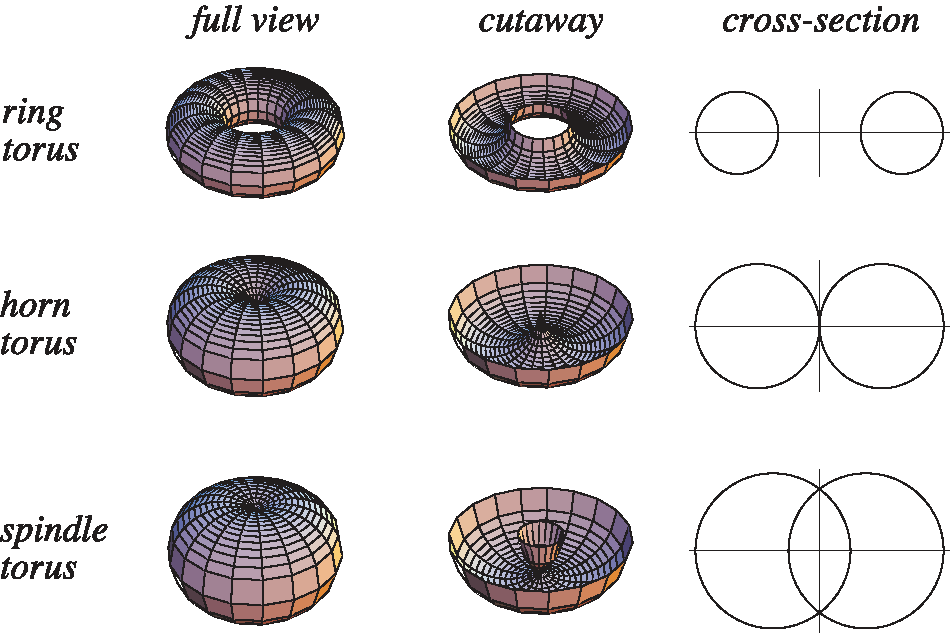
\includegraphics[width=0.7\linewidth]{pic/StandardTori701.pdf}
        \caption{StandardTori701}
        \label{fig:StandardTori701}
    \end{figure}
    If we think of $\mathbf{N} = \mathbf{N}(u, v)$ as a directed line segment, 
    pointing from $\Phi(u, v)$ to $\Phi(u, v) + \mathbf{N}(u, v)$, 
    then $\mathbf{N}$ points outward, 
    that is to say, away from $\Psi(K)$. 
    This is so because $\mathbf{J}_{\Psi} > 0$ when $t = a$.

    For example, take $u = v = \pi/2$, $t = a$. 
    This gives the largest value of $z$ on $\Psi(K)$, 
    and $\mathbf{N} = a(b + a)\mathbf{e}_3$ points ``upward'' for this choice of $(u, v)$.
\end{newexample}

\begin{mydef}
    \label{mydef:10.48}
    \myKeyword{Integrals of 1-forms in $\R^3$}
    Let $\gamma$ be a $\mathscr{C}'$-curve in an open set $E \subset \R^3$, with parameter interval $[0, 1]$, 
    let $\mathbf{F}$ be a vector field in $E$, as in Sec. \ref{mydef:10.42}, 
    and define $\lambda_{\mathbf{F}}$, by \eqref{eq:10.124}. 
    The integral of $\lambda_{\mathbf{F}}$, over $\gamma$ can be rewritten in a certain way which we now describe.

    For any $u \in [0,1]$,
    \begin{equation*}
        \gamma' (u) = 
        \gamma'_1 (u) \mathbf{e}_1 +
        \gamma'_2 (u) \mathbf{e}_2 +
        \gamma'_3 (u) \mathbf{e}_3 
    \end{equation*}
    is called the \myKeyword{tangent vector} to $\gamma$ at $u$. 
    We define $\mathbf{t} = \mathbf{t}(u)$ to be the unit vector in the direction of $\gamma'(u)$. 
    Thus
    \begin{equation*}
        \gamma'(u) = \left| \gamma'(u) \right| \mathbf{t} (u) .
    \end{equation*}
    [If $\gamma'(u) = \mathbf{0}$ for some $u$, 
    put $\mathbf{t}(u) = \mathbf{e}_1$; 
    any other choice would do just as well.]
    By \eqref{eq:10.35},
    \begin{equation}
        \label{eq:10.142}
        \begin{aligned}
            \int_{\gamma} \lambda_{\mathbf{F}}
            &= \sum_{i=1}^{3} \int_{0}^{1} F_i (\gamma(u)) \gamma'_i(u) \d u \\
            &= \int_{0}^{1} \mathbf{F} (\gamma(u)) \cdot \gamma'(u) \d u \\
            &= \int_{0}^{1} \mathbf{F} (\gamma(u)) \cdot \mathbf{t}(u) \left| \gamma'(u) \right| \d u .
        \end{aligned}
    \end{equation}

    Theorem \ref{thm:6.27} makes it reasonable to call $| \gamma'(u) | \d u$ the \myKeywordblue{element of arc length along} $\gamma$. 
    A customary notation for it is $\d s$, and \eqref{eq:10.142} is rewritten in the form
    \begin{equation}
        \label{eq:10.143}
        \int_{\gamma} \lambda_{\mathbf{F}}
        = \int_{\gamma} (\mathbf{F \cdot t}) \d s .
    \end{equation}

    Since $\mathbf{t}$ is a unit tangent vector to $\gamma$, 
    $\mathbf{F \cdot t}$ is called the \myKeywordblue{tangential component} of $\mathbf{F}$ along $\gamma$.

    The right side of \eqref{eq:10.143} should be regarded as just an abbreviation for the last integral in \eqref{eq:10.142}. 
    The point is that $\mathbf{F}$ is defined on the range of $\gamma$, but $\mathbf{t}$ is defined on $[0, 1]$; 
    thus $\mathbf{F \cdot t}$ has to be properly interpreted. 
    Of course, when $\gamma$ is one-to-one, 
    then $\mathbf{t}(u)$ can be replaced by $\mathbf{t}(y(u))$, and this difficulty disappears.
\end{mydef}

\begin{mydef}
    \label{mydef:10.49}
    \myKeyword{Integrals of 2-forms in $\R^3$}
    Let $\Phi$ be a 2-surface in an open set $E \subset \R^3$,
    of class $\mathscr{C}'$, with parameter domain $D \subset \R^2$. 
    Let $\mathbf{F}$ be a vector field in $E$, and define $\omega_{\mathbf{F}}$ by \eqref{eq:10.125}. 
    As in the preceding section, we shall obtain a different representation of the integral of $\omega_{\mathbf{F}}$ over $\Phi$.

    By \eqref{eq:10.35} and \eqref{eq:10.129},
    \begin{align*}
        \int_{\Phi} \omega_{\mathbf{F}} 
        &= \int_{\Phi} \left( 
            F_1 \d y \wedge \d z + 
            F_2 \d z \wedge \d x + 
            F_3 \d x \wedge \d y  
            \right) \\
        &= \int_{D} \left\{ 
            (F_1 \circ \Phi) \frac{\partial (y,z)}{\partial (u,v)} + 
            (F_2 \circ \Phi) \frac{\partial (z,x)}{\partial (u,v)} + 
            (F_3 \circ \Phi) \frac{\partial (x,y)}{\partial (u,v)} 
         \right\} \d u \d v \\
        &= \int_{D} \mathbf{F}(\Phi(u,v))\cdot \mathbf{N}(u,v) \d u \d v .
    \end{align*}
    Now let $\mathbf{n} = \mathbf{n}(u, v)$ be the unit vector in the direction of $\mathbf{N}(u, v)$. 
    [If $\mathbf{N}(u, v) = 0$ for some $(u, v) \in D$, 
    take $\mathbf{n}(u, v) = \mathbf{e}_1$.] 
    Then $\mathbf{N = |N |n}$, and therefore the last integral becomes
    \begin{equation*}
        \int_{D} \mathbf{F}(\Phi(u,v)\cdot \mathbf{n}(u,v))
        \left| \mathbf{N}(u,v) \right| \d u \d v .
    \end{equation*}
    By \eqref{eq:10.131}, we can finally write this in the form
    \begin{equation}
        \label{eq:10.144}
        \int_{\Phi} \omega_{\mathbf{F}} = 
        \int_{\Phi} (\mathbf{F \cdot n}) \d A .
    \end{equation}
    With regard to the meaning of $\mathbf{F \cdot n}$, 
    the remark made at the end of Sec. \ref{mydef:10.48} applies here as well.
\end{mydef}

We can now state the original form of Stokes' theorem.

\begin{thm}
    \label{thm:10.50}
    \myKeyword{Stokes' formula}
    If $\mathbf{F}$ is a vector field of class $\mathscr{C}'$ in an open set $E \subset \R^3$, 
    and if $\Phi$ is a 2-surface of class $\mathscr{C}''$ in $E$, then
    \begin{equation}
        \label{eq:10.145}
        \int_{\Phi} \left( \nabla \times \mathbf{F} \right) \cdot \mathbf{n} \d A = 
        \int_{\partial \Phi} \left( \mathbf{F \cdot t} \right)  \d s
    \end{equation}
\end{thm}

\begin{proof}
    Put $\mathbf{H} = \nabla \times \mathbf{F}$.
    Then, as in the proof of Theorem \ref{thm:10.43},
    we have 
    \begin{equation}
        \label{eq:10.146}
        \omega_{\mathbf{H}} = \d \lambda_{\mathbf{F}} . 
    \end{equation}
    Hence 
    \begin{align*}
        \int_{\Phi} (\nabla \times \mathbf{F}) \cdot \mathbf{n} \d A 
        &= \int_{\Phi} (\mathbf{H \cdot n}) \d A 
        = \int_{\Phi} \omega_{\mathbf{H}} \\
        &= \int_{\Phi} \d \lambda_{\mathbf{F}} 
        = \int_{\partial \Phi} \lambda_{\mathbf{F}} 
        = \int_{\partial \Phi} (\mathbf{F \cdot t}) \d s .
    \end{align*}
    Here we used the definition of $\mathbf{H}$, 
    then \eqref{eq:10.144} with $\mathbf{H}$ in place of $\mathbf{F}$, 
    then \eqref{eq:10.146}, then-the main step-Theorem \ref{thm:10.33}, 
    and finally \eqref{eq:10.143}, extended in the obvious way from curves to 1-chains.
\end{proof}

\begin{thm}
    \label{thm:10.51}
    \myKeyword{The divergence theorem}
    If $\mathbf{F}$ is a vector field of class $\mathscr{C}'$ in an open set $E \subset \R^3$, 
    and if $\Omega$ is a closed subset of $E$ with positively oriented boundary $\partial \Omega$ (as described in Sec. \ref{mydef:10.31}) then
    \begin{equation}
        \label{eq:10.147}
        \int_{\Omega} \left( \nabla \cdot \mathbf{F} \right) \d V 
        \int_{\partial \Omega} \left( \mathbf{F} \cdot \mathbf{n} \right) \d A . 
    \end{equation}
\end{thm}

\begin{proof}
    By \eqref{eq:10.125}
    \begin{equation*}
        \d \omega_{\mathbf{F}} = 
        (\nabla \cdot \mathbf{F}) \d x \wedge \d y \wedge \d z = 
        (\nabla \cdot \mathbf{F}) \d V .
    \end{equation*}
    Hence 
    \begin{equation*}
        \int_{\Omega} (\nabla \cdot \mathbf{F}) \d V
        = \int_{\Omega} \d \omega_{\mathbf{F}} 
        = \int_{\partial \Omega} \omega_{\mathbf{F}} 
        = \int_{\partial \Omega} (\mathbf{F \cdot n}) \d A ,
    \end{equation*}
    by Theorem \ref{thm:10.33}, 
    applied to the 2-form $\omega_{\mathbf{F}}$, and \eqref{eq:10.144}.
\end{proof}

% chap10exercise

\section{Exercises}


\begin{myexercise}
    \label{ex:10.1}
    Let $H$ be a compact convex set in $\R^k$, with nonempty interior.
    Let $f \in \mathscr{C}(H)$, put $f(\mathbf{x}) = 0$ in the complement of $H$,
    and define $\int_H f$ as in Definition \ref{mydef:10.3}.

    Prove that $\int_H f$ is independent of the order in which the $k$ integrations are carried out.

    \emph{Hint:} Approximate $f$ by functions that are continuous on $\R^k$ and whose supports are in $H$, as was done in Example \ref{newexample:10.47}.
\end{myexercise}


\begin{myexercise}
    \label{ex:10.2}
    For $i = 1, 2, 3, ...$ , let $\phi_i \in \mathscr{C}(\R^1)$ have support in $(2^{-i} , 2^{1-i})$, such that $\int \phi_i = 1$.
    Put
    \begin{equation*}
        f(x,y) = \sum_{i=1}^{\infty}
        \left[
            \phi_{i}(x) -
            \phi_{i+1}(x)
            \right] \phi_i (y)
    \end{equation*}
    Then $f$ has compact support in $\R^2$,
    $f$ is continuous except at $(0,0)$,
    and
    \begin{equation*}
        \int \d y \int f(x,y) \d x = 0
        \quad \text{ but } \quad
        \int \d x \int f(x,y) \d y = 1.
    \end{equation*}
    Observe that $f$ is unbounded in every neighborhood of $(0, 0)$.
\end{myexercise}


\begin{myexercise}
    \label{ex:10.3}
    \begin{asparaenum}[(a)]
        \item If $F$ is as in Theorem \ref{thm:10.7}, put
        $\mathbf{A} = \mathbf{F}'(0)$,
        $\mathbf{F_{1}(x)} = \mathbf{A^{-1}F(x)}$.
        Then $\mathbf{F'_1(0)}=I$.
        Show that
        \begin{equation*}
            \mathbf{F_1(x) = G_n \circ G_{n-1} \circ \cdots \circ G_1(x)}
        \end{equation*}
        in some neighborhood of $\mathbf{0}$,
        for certain primitive mappings $\mathbf{G_n \circ \cdots \circ G_1(x)}$.
        This gives another version of Theorem \ref{thm:10.7}:
        \begin{equation*}
            \mathbf{F(x) = F'(0) G_n \circ G_{n-1} \circ \cdots \circ G_1(x)}.
        \end{equation*}
        \item Prove that the mapping $(x, y) > (y, x)$ of $\R^2$ onto $\R^2$ is not the composition of any two primitive mappings, in any neighborhood of the origin.
        (This shows that the flips $B_1$ cannot be omitted from the statement of Theorem \ref{thm:10.7}.)
    \end{asparaenum}
\end{myexercise}

\begin{myexercise}
    \label{ex:10.4}
    For $(x,y) \in \R^2$, define
    \begin{equation*}
        \mathbf{F}(x,y) = (e^x \cos y - 1, e^x \sin y).
    \end{equation*}
    Prove that $\mathbf{F = G_2 \circ G_1}$, where
    \begin{align*}
        \mathbf{G}_1 (x,y) & = (e^x \cos y - 1, y) \\
        \mathbf{G}_2 (u,v) & = (u, (1 + u) \tan v)
    \end{align*}
    are primitive in some neighborhood of $(0, 0)$.

    Compute the Jacobians of $\mathbf{G_1, G_2, F}$ at $(0, 0)$.
    Define
    \begin{equation*}
        \mathbf{H}_2 (x,y) = (x, e^x \sin y)
    \end{equation*}
    and find
    \begin{equation*}
        \mathbf{H}_1 (u,v) = (h(u,v), v)
    \end{equation*}
    so that $\mathbf{F = H_1 \circ H_2}$ is some neighborhood of $(0,0)$.
\end{myexercise}


\begin{myexercise}
    \label{ex:10.5}
    Formulate and prove an analogue of Theorem \ref{thm:10.8},
    in which $K$ is a compact subset of an arbitrary metric space.
    (Replace the functions $\phi_i$ that occur in the
    proof of Theorem \ref{thm:10.8}
    by functions of the type constructed in Exercise \ref{ex:4.22})
\end{myexercise}


\begin{myexercise}
    \label{ex:10.6}
    Strengthen the conclusion of Theorem \ref{thm:10.8} by showing that the functions $\psi_i$ can be made differentiable, and even infinitely differentiable.
    (Use Exercise \ref{ex:8.1} in the construction of the auxiliary functions $\phi_i$.)
\end{myexercise}


\begin{myexercise}
    \label{ex:10.7}
    \begin{enumerate}[(a)]
        \item Show that the simplex $Q^k$ is the smallest convex subset of $\R^k$ that contains $\mathbf{0},\mathbf{e}_1,\dots,\mathbf{e}_k$.
        \item Show that affine mappings take convex sets to convex sets.
    \end{enumerate}
\end{myexercise}


\begin{myexercise}
    \label{ex:10.8}
    Let $H$ be the parallelogram in $\R^2$ whose vertices are $(1, 1), (3, 2), (4, 5), (2, 4)$.
    Find the affine map $T$ which sends $(0, 0)$ to $(1, 1)$, $(1, 0)$ to $(3, 2)$, $(0, 1)$ to $(2, 4)$.
    Show that $J_T = 5$.
    Use $T$ to convert the integral
    \begin{equation*}
        \alpha = \int_H e^{x-y} \d x \d y
    \end{equation*}
    to an integral over $I^2$ and thus compute $\alpha$.
\end{myexercise}


\begin{myexercise}
    \label{ex:10.9}
    Define $(x, y) = T(r, \theta)$ on the rectangle
    \begin{equation*}
        0 \leq r \leq a,
        \quad
        0 \leq \theta \leq 2\pi
    \end{equation*}
    by the equations
    \begin{equation*}
        x = r \cos \theta , \quad
        y = r \sin \theta .
    \end{equation*}
    Show that $T$ maps this rectangle onto the closed disc $D$ with center at $(0, 0)$ and radius $a$,
    that $T$ is one-to-one in the interior of the rectangle, and that $J_T(r, \theta) = r$.
    If $f \in \mathscr{C}(D)$, prove the formula for integration in polar coordinates:
    \begin{equation*}
        \int_D f(x,y) \d x \d y =
        \int_{0}^{a} \int_{0}^{2\pi} f(T(r,\theta)) r \d r \d \theta .
    \end{equation*}
    \emph{Hint:} Let Do be the interior of $D$, minus the interval from $(0, 0)$ to $(0, a)$.
    As it stands, Theorem \ref{thm:10.9} applies to continuous functions $f$ whose support lies in $D_0$.
    To remove this restriction, proceed as in Example \ref{newexample:10.4}.
\end{myexercise}



\begin{myexercise}
    \label{ex:10.10}
    Let $a \rightarrow \infty$ in \ref{ex:11.9} and prove that
    \begin{equation*}
        \int_{\R^2} f(x,y) \d x \d y =
        \int_{0}^{\infty} \int_{0}^{2\pi} f(T(r,\theta)) r \d r \d \theta ,
    \end{equation*}
    for continuous functions f that decrease sufficiently rapidly as $|x | + | y | \rightarrow \infty$.
    (Find a more precise formulation.)
    Apply this to
    \begin{equation*}
        f(x, y) = \exp (-x^2 - y^2)
    \end{equation*}
    to derive formula \eqref{eq:8.101}.
\end{myexercise}


\begin{myexercise}
    \label{ex:10.11}
    Define $(u,v)=T(s,t)$ on the strip
    \begin{equation*}
        0<s<\infty , \quad
        0<t<1
    \end{equation*}
    by setting $u = s - st$, $v = st$.
    Show that $T$ is a 1-1 mapping of the strip onto the positive quadrant $Q$ in $\R^2$.
    Show that $J_T(s, t) = s$.

    For x > 0, y > 0, integrate
    \begin{equation*}
        u^{x-1} e^{-u} v^{y-1} e^{-v}
    \end{equation*}
    over $Q$, use Theorem \ref{thm:10.9} to convert the integral to one over the strip, and derive formula \eqref{eq:8.96} in this way.
    (For this application, Theorem \ref{thm:10.9} has to be extended so as to cover certain improper integrals.
    Provide this extension.)
\end{myexercise}


\begin{myexercise}
    \label{ex:10.12}
    Let $I^k$ be the set of all $\mathbf{u} = (u_1, ... , u_k) \in \R^k$ with $0 \leq u_i \leq 1$ for all $i$;
    let $Q^k$ be the set of all $\mathbf{x} = (x_1, ... , x_k) \in  \R^k$ with $x_i \geq 0, \sum x_i \leq 1$.
    ($I^k$ is the unit cube;
    $Q^k$ is the standard simplex in $\R^k$.)
    Define $\mathbf{x} = T(\mathbf{u})$ by
    \begin{align*}
        x_1   & = u_1                          \\
        x_2   & = (1-u_1)u_2                   \\
        \dots & \dots
        x_k   & = (1-u_1)\cdots(1-u_{k-1})u_k.
    \end{align*}
    Show that
    \begin{equation*}
        \sum_{i=1}^{k} x_i = 1 - \prod_{i=1}^{k} (1-u_i) .
    \end{equation*}

    Show that $T$ maps $I^k$ onto $Q^k$,
    that $T$ is 1-1 in the interior of $I^k$,
    and that its inverse $S$ is defined in the interior of $Q^k$ by $u_1 = x_1$ and
    \begin{equation*}
        u_i = \frac{x_i}{1-x_1-\cdots-x_{i-1}}
    \end{equation*}
    for $i=2,\dots,k$.
    Show that
    \begin{equation*}
        J_T(\mathbf{u}) =
        (1-u_1)^{k-1}
        (1-u_2)^{k-2}
        \cdots
        (1-u_{k-1}),
    \end{equation*}
    and
    \begin{equation*}
        J_S(\mathbf{x}) =
        \left[
            (1-x_1)
            (1-x_1-x_2)
            \cdots
            (1-x_1-\cdots-x_{k-1})
            \right]^{-1} .
    \end{equation*}
\end{myexercise}


\begin{myexercise}
    \label{ex:10.13}
    Let $r_1,\dots,r_k$ be nonnegative integers, and prove that
    \begin{equation*}
        \int_{Q^k}
        x_1^{r_1}
        \cdots
        x_k^{r_k}
        \d x =
        \frac{r_1!\cdots r_k!}{(k+r_1+\cdots+r_k)!}
    \end{equation*}
    \emph{Hint:} Use Exercise \ref{ex:11.12}, Theorem \ref{thm:10.9} and \ref{thm:8.20}.

    Note that the special case $r_1 = \cdots = r_k = 0$
    shows that the volume of $Q^k$ is $1/k!$.
\end{myexercise}


\begin{myexercise}
    \label{ex:10.14}
    Prove formula \eqref{eq:10.46}.
\end{myexercise}


\begin{myexercise}
    \label{ex:10.15}
    If $\omega$ and $\lambda$ are $k$- and $m$-forms, respectively, prove that
    \begin{equation*}
        \omega \wedge \lambda =
        (-1)^{km} \lambda \wedge \omega .
    \end{equation*}
\end{myexercise}


\begin{myexercise}
    \label{ex:10.16}
    If $k \geq 2$ and $\delta = [\mathbf{p}_0, \mathbf{p}_1, ... , \mathbf{p}_t]$ is an oriented affine $k$-simplex,
    prove that $\partial^2 \sigma = 0$,
    directly from the definition of the boundary operator $\partial$.
    Deduce from this that $\partial^2 \Psi = 0$ for every chain $\Psi$.

    \emph{Hint:} For orientation, do it first for $k= 2, k = 3$.
    In general, if $i <j$, let $\sigma_{ij}$ be the $(k - 2)$-simplex obtained by deleting $\mathbf{p}_i$ and $\mathbf{p}_j$ from $u$.
    Show that each $\sigma_{ij}$ occurs twice in $\partial^2 \sigma$, with opposite sign.
\end{myexercise}


\begin{myexercise}
    \label{ex:10.17}
    Put $J^2 = \tau_1 + \tau_2$, where
    \begin{equation*}
        \tau_1 =  \left[ \mathbf{0,e_1,e_1+e_2} \right],
        \quad
        \tau_2 = -\left[ \mathbf{0,e_2,e_2+e_1} \right].
    \end{equation*}
    Explain why it is reasonable to call $J^2$ the positively oriented unit square in $\R^2$ .
    Show that $\partial J^2$ is the sum of 4 oriented affine 1-simplexes. Find these. What is $\partial (\tau_1 - \tau_2)$?
\end{myexercise}


\begin{myexercise}
    \label{ex:10.18}
    Consider the oriented affine 3-simplex
    \begin{equation*}
        \sigma_1 =  \left[ \mathbf{0,e_1,e_1+e_2,e_1+e_2+e_3} \right]
    \end{equation*}
    in $\R^3$.
    Show that $\sigma_1$
    (regarded as a linear transformation) has determinant 1.
    Thus $\sigma_1$ is positively oriented.

    Let $\sigma_2 , ... , \sigma_6$ be five other oriented 3-simplexes, obtained as follows:
    There are five permutations $(i_1, i_2, i_3)$ of $(1, 2, 3)$, distinct from $(1, 2, 3)$.
    Associate with each $(i_1, i_2, i_3)$ the simplex
    \begin{equation*}
        s(i_1, i_2, i_3) \left[ \mathbf{0,e_{i_1},e_1+e_2} \right]
    \end{equation*}
    where $s$ is the sign that occurs in the definition of the determinant.
    (This is how $\tau_2$ was obtained from $\tau_1$ in Exercise \ref{ex:11.17}.)

    Show that $\sigma_2, \dots , \sigma_6$ are positively oriented.

    Put $J^3 = \sigma_1 + \dots + \sigma_6$.
    Then $J^3$ may be called the positively oriented unit cube in $\R^3$.

    Show that $\partial J^3$ is the sum of 12 oriented affine 2-simplexes.
    (These 12 triangles cover the surface of the unit cube $I^3$,)

    Show that $\mathbf{x} = (\mathbf{x}_1, \mathbf{x}_2, \mathbf{x}_3)$ is in the range of $\sigma_1$ if and only if $0 \leq x_3 \leq x_2 \leq x_1 \leq 1$,

    Show that the ranges of $\sigma_1, ... , \sigma_6$ have disjoint interiors, and that their union covers $I^3$.
    (Compare with Exercise \ref{ex:11.13}; note that $3! = 6$.)
\end{myexercise}


\begin{myexercise}
    \label{ex:10.19}
    Let $J^2$ and $J^3$ be as in Exercise \ref{ex:11.17} and \ref{ex:11.18}.
    Define
    \begin{align*}
        B_{01}(u,v) = (0,u,v), & B_{11}(u,v) = (1,u,v), \\
        B_{02}(u,v) = (u,0,v), & B_{12}(u,v) = (u,1,v), \\
        B_{03}(u,v) = (u,v,0), & B_{13}(u,v) = (u,v,1), \\
    \end{align*}
    These are affine, and map $\R^2$ into $\R^3$.

    Put $\beta_{ri} = B_{ri}(J^2)$, for $r = 0,1$, $i=1,2,3$.
    Each $\beta_{ri}$ is an affine-oriented 2-chain.
    (See Sec. \ref{mydef:10.30}.)
    Verify that
    \begin{equation*}
        \partial J^3 = \sum_{i=1}^{3}(-1)^i (\beta_{0i}-\beta_{1i}),
    \end{equation*}
    in agreement with Exercise \ref{ex:10.18}.
\end{myexercise}



\begin{myexercise}
    \label{ex:10.20}
    State conditions under which the formula
    \begin{equation*}
        \int_{\Phi} f \d \omega =
        \int_{\partial\Phi} f \omega -
        \int_{\Phi} (\d f) \wedge \omega
    \end{equation*}
    is valid, and show that it generalizes the formula for integration by parts.

    \emph{Hint:} $\d(f \omega) = (\d f) \wedge \omega + f d\omega$.
\end{myexercise}


\begin{myexercise}
    \label{ex:10.21}
    As in Example \ref{newexample:10.36}, consider the 1-form
    \begin{equation*}
        \eta = \frac{x \d y - y \d x}{x^2+y^2}
    \end{equation*}
    in $\R^2 - \{\mathbf{0}\}$.
    \begin{asparaenum}[(a)]
        \item Carry out the computation that leads to formula \eqref{eq:10.113}, and prove that $\d \eta = 0$.
        \item Let $\gamma(t) = (r \cos t, r \sin t)$, for some $r > 0$,
        and let $r$ be a $\mathscr{C}''$-curve in $\R^2 - \{\mathbf{0}\}$,
        with parameter interval $[0, 2\pi]$, with $\Gamma(0) = \Gamma(2\pi)$, such that the intervals $[\gamma(t), \Gamma(t)]$ do not contain $\mathbf{0}$ for any $t \in $$[0, 2\pi]$. Prove that
            \begin{equation*}
                \int_{\Gamma} \eta = 2 \pi .
            \end{equation*}

            \emph{Hint:} For $0 \leq t \leq 2\pi$, $0 \leq u \leq 1$, define
            \begin{equation*}
                \Phi(t,u)=(1-u)\Gamma(t)+u\gamma(t).
            \end{equation*}
            Then $\Phi$ is a 2-surface in $\R^2 - \{\mathbf{0}\}$ whose parameter domain is the indicated rectangle.
            Because of cancellations (as in Example \ref{newexample:10.32}),
            \begin{equation*}
                \partial \Phi = \Gamma - \gamma .
            \end{equation*}
            Use Stokes' theorem to deduce that
            \begin{equation*}
                \int_{\Gamma} \eta =
                \int_{\gamma} \eta
            \end{equation*}
            because $\d \eta = 0$.
            \item Take $\Gamma(t)=(a \cos t, b \sin t)$ where $a>0,b>0$ are fixed. Use part (b) to show that
            \begin{equation*}
                \int_{0}^{2\pi} \frac{ab}{a^2\cos^2 t + b^2 \sin^2 t} \d t = 2 \pi .
            \end{equation*}
            \item Show that
            \begin{equation*}
                \eta = \d \left( \arctan\frac{y}{x} \right)
            \end{equation*}
            in any convex open set in which $x \neq 0$, and that
            \begin{equation*}
                \eta = \d \left( -\arctan\frac{x}{y} \right)
            \end{equation*}
            in any convex open set in which $y \neq 0$.
            \item Show that (b) can be derived from (d).
            \item If $\Gamma$ is any closed $\mathscr{C}'$-curve in $\R^2 - \{\mathbf{0}\}$, prove that
        \begin{equation*}
            \frac{1}{2\pi} \int_{\Gamma} \eta = \Ind (\Gamma).
        \end{equation*}
        (See Exercise \ref{ex:8.23} for the definition of the index of a curve.)
    \end{asparaenum}
\end{myexercise}


\begin{myexercise}
    \label{ex:10.22}
    As in Example \ref{newexample:10.37}, define $\zeta$ in $\R^3 - \{\mathbf{0}\}$ by
    \begin{equation*}
        \zeta =
        \frac{
            x \d y \wedge \d z +
            y \d z \wedge \d x +
            z \d x \wedge \d y
        }{r^3}
    \end{equation*}
    where $r = \left( x^2+y^2+z^2 \right)^{1/2}$,
    let $D$ be the rectangle given by
    $0 \leq u \leq \pi$,
    $0 \leq v \leq \pi$,
    and let $\sum$ be the 2-surface in $\R^3$,
    with parameter domain in $D$, given by
    \begin{equation*}
        x = \sin u \cos v, \quad
        y = \sin u \sin v, \quad
        z = \cos u .
    \end{equation*}
    \begin{asparaenum}[(a)]
        \item Prove that $\d \zeta = 0$ in $\R^3 - \{\mathbf{0}\}$.
        \item Let $S$ denote the restriction of $\sum$ to a parameter domain $E \subset D$.
        Prove that
        \begin{equation*}
            \int_S \zeta = \int_E \sin u \d u \d v = A(S),
        \end{equation*}
        where $A$ denotes area, as in Sec. \ref{thm:10.43}.
        Note that this contains \eqref{eq:10.115} as a special case.
        \item Suppose $g, h_1, h_2, h_3$, are $\mathscr{C}''$-functions on $[0, 1], g > 0$.
        Let $(x, y, z) = \Phi(s, t)$
        define a 2-surface $\Phi$, with parameter domain $I^2$, by
        \begin{equation*}
            x = g(t)h_1(s) , \quad
            y = g(t)h_2(s) , \quad
            z = g(t)h_3(s) .
        \end{equation*}
        Prove that
        \begin{equation*}
            \int_{\Phi} \zeta = 0 ,
        \end{equation*}
        directly from \eqref{eq:10.35}.

        Note the shape of the range of $\Phi$:
        For fixed $s$, $\Phi(s, t)$ runs over an interval on a line through 0.
        The range of $\Phi$ thus lies in a ``cone'' with vertex at the origin.
        \item Let $E$ be a closed rectangle in $D$, with edges parallel to those of $D$.
        Suppose $f \in \mathscr{C}''(D), f> 0$.
        Let $\Omega$ be the 2-surface with parameter domain $E$, defined by
        \begin{equation*}
            \Omega(u,v) = f(u,v)\sum(u,v).
        \end{equation*}
        Define $S$ as in (b) and prove that
        \begin{equation*}
            \int_{\Phi} \zeta =  \int_{S} \zeta = A(S).
        \end{equation*}
        (Since $S$ is the ``radial projection'' of $n$ into the unit sphere, this result makes it reasonable to call $\int_n \zeta$ the ``solid angle'' subtended by the range of $\Omega$ at the origin.)

        \emph{Hint:} Consider the 3-surface $\Psi$ given by
        \begin{equation*}
            \Psi(t,u,v) = \left[ 1-t+t f(u,v) \right] \sum (u,v) ,
        \end{equation*}
        where $(u, v) \in E$, $0 \leq t \leq 1$.
        For fixed $v$, the mapping $(t, u) \rightarrow \Psi(t, u, v)$ is a 2-surface $\Psi$ to which (c) can be applied to show that $\int_{\Phi} \zeta = 0$.
        The same thing holds when $u$ is fixed.
        By (a) and Stokes' theorem,
        \begin{equation*}
            \int_{\partial \Psi} \zeta =
            \int_{\Psi} \d \zeta = 0.
        \end{equation*}
        \item Put $\lambda = -(z/r)\eta$, where
        \begin{equation*}
            \eta = \frac{x \d y - y \d x}{x^2+y^2} ,
        \end{equation*}
        as in Exercise \ref{ex:10.21}.
        Then $\lambda$ is a 1-form in the open set $V \subset \R^3$ in which $x^2 + y^2 > 0$.
        Show that $\zeta$ is \myKeywordblue{exact in} $V$ by showing that
        \begin{equation*}
            \zeta = \d \lambda .
        \end{equation*}
        \item Derive (d) from (e), without using (c).
        \emph{Hint:} To begin with, assume $0 < u < \pi$ on $E$.
        By (e),
        \begin{equation*}
            \int_{\Omega} \zeta = \int_{\partial \Omega} \lambda
            \quad \text{ and } \quad
            \int_{S} \zeta = \int_{\partial S} \lambda .
        \end{equation*}
        Show that the two integrals of $\lambda$ are equal, by using part (d) of Exercise \ref{ex:10.21},
        and by noting that $z/r$ is the same at $\sum(u, v)$ as at $\Omega(u, v)$.
        \item Is $\zeta$ exact in the complement of every line through the origin?
    \end{asparaenum}
\end{myexercise}


\begin{myexercise}
    \label{ex:10.23}
    Fix $n$.
    Define $r_k = (x_1^2 + \cdots + x_k^2)$ for $1 \leq k \leq n$, let $E_k$ be the set of all $\mathbf{x} \in \R^n$ at which $r_k > 0$, and let $\omega_k$ be the $(k - 1)$-form defined in $E_k$ by
    \begin{equation*}
        \omega_k = (r_k)^{-k} \sum_{i=1}^{k} (-1)^{i-1} x_i
        \d x_1 \wedge \cdots \wedge
        \d x_{i-1} \wedge
        \d x_{i+1} \wedge \cdots \wedge
        \d x_k .
    \end{equation*}
    Note that $\omega_2 = \eta$, $\omega_3 = \zeta$, in the terminology of Exercises \ref{ex:10.21} and \ref{ex:10.22}.
    Note also that
    \begin{equation*}
        E_1 \subset
        E_2 \subset
        \cdots \subset
        E_n = \R^n - \{\mathbf{0}\} .
    \end{equation*}
    \begin{asparaenum}[(a)]
        \item Prove that $\d \omega_k = 0$ in $E_k$.
        \item For $k=2,\dots,n$, prove that $\omega_k$ is exact in $E_{k-1}$, by showing that
        \begin{equation*}
            \omega_k = \d (f_k \omega_{k-1})
            = (\d f_k) \wedge \omega_{k-1} ,
        \end{equation*}
        where $f_k(\mathbf{x})=(-1)^k g_k(x_k/r_k)$ and
        \begin{equation*}
            g_k(t)=\int_{-1}^{t}(1-s^2)^{(k-3)/2} \d s
            \quad (-1<t<1).
        \end{equation*}
        \emph{Hint:} $f_k$ satisfies the differential equations
        \begin{equation*}
            \mathbf{x} \cdot (\nabla f_k)(\mathbf{x}) = 0
        \end{equation*}
        and
        \begin{equation*}
            (D_k f_k)(\mathbf{x}) = \frac{(-1)^k(r_{k-1})^{k-1}}{(r_k)^k}.
        \end{equation*}
        \item Is $\omega_n$ exact in $E_n$?
        \item Note that (b) is a generalization of part (e) of Exercise \ref{ex:10.22}.
        Try to extend some of the other assertions of Exercises \ref{ex:10.21} and \ref{ex:10.22} to $\omega_n$, for arbitrary $n$.
    \end{asparaenum}
\end{myexercise}


\begin{myexercise}
    \label{ex:10.24}
    Let $\omega = \sum a_i(\mathbf{x}) \d x_i$ be a 1-form of class $\mathscr{C}''$ in a convex open set $E \subset \R^n$.
    Assume $\d \omega = 0$ and prove that $\omega$ is exact in $E$, by completing the following outline:

    Fix $\mathbf{p} \in E$.
    Define
    \begin{equation*}
        f(\mathbf{x}) = \int_{[\mathbf{p,x}]} \omega
        \quad
        (\mathbf{x} \in E).
    \end{equation*}
    Apply Stokes' theorem to affine-oriented 2-simplexes $[\mathbf{p, x, y}]$ in $E$.
    Deduce that
    \begin{equation*}
        f(\mathbf{y}) -
        f(\mathbf{x}) =
        \sum_{i=1}^{n} (y_i-x_i)
        \int_{0}^{1} a_i ((1-t)\mathbf{x}+t\mathbf{y}) \d \mathbf{t}
    \end{equation*}
    for
    $\mathbf{x} \in E$ ,
    $\mathbf{y} \in E$ .
    Hence $(D_i f)(\mathbf{x}) = a_i(\mathbf{x})$.
\end{myexercise}


\begin{myexercise}
    \label{ex:10.25}
    Assume that $\omega$ is a 1-form in an open set $E \subset \R^n$ such that
    \begin{equation*}
        \int_{\gamma} \omega = 0
    \end{equation*}
    for every closed curve $\gamma$ in $E$, of class $\mathscr{C}'$.
    Prove that $\omega$ is exact in $E$, by imitating part of the argument sketched in Exercise \ref{ex:10.24}.
\end{myexercise}


\begin{myexercise}
    \label{ex:10.26}
    Assume $\omega$ is a 1-form in $\R^3-\{\mathbf{0}\}$, of class $\mathscr{C}'$ and $\d \omega =0$.
    Prove that w is exact in $\R^3-\{\mathbf{0}\}$.

    \emph{Hint:} Every closed continuously differentiable curve in $\R^3-\{\mathbf{0}\}$ is the boundary of a 2-surface in $\R^3-\{\mathbf{0}\}$.
    Apply Stokes' theorem and Exercise \ref{ex:10.25}.
\end{myexercise}


\begin{myexercise}
    \label{ex:10.27}
    Let $E$ be an open 3-cell in $\R^3$, with edges parallel to the coordinate axes.
    Suppose $(a, b, c) \in E$, $f_i \in \mathscr{C}'(E)$ for $i = 1, 2, 3$,
    \begin{equation*}
        \omega =
        f_1 \d y \wedge \d z +
        f_2 \d z \wedge \d x +
        f_3 \d x \wedge \d y ,
    \end{equation*}
    and assume that $\d \omega = 0$ in $E$.
    Define
    \begin{equation*}
        \lambda = g_1 \d x + g_2 \d y
    \end{equation*}
    where
    \begin{align*}
        g_1(x,y,z) & = \int_{c}^{z} f_2(x,y,s) \d s - \int_{b}^{y} f_3(x,t,c) \d t \\
        g_2(x,y,z) & = -\int_{c}^{z} f_1(x,y,s) \d s ,
    \end{align*}
    for $(x, y, z) \in E$.
    Prove that $\d \lambda = \omega$ in $E$.

    Evaluate these integrals when $\omega = \zeta$ and thus find the form $\lambda$ that occurs in part (e) of Exercise \ref{ex:10.22}.
\end{myexercise}


\begin{myexercise}
    \label{ex:10.28}
    Fix $b > a > 0$, define
    \begin{equation*}
        \Phi(r, \theta) = (r \cos \theta, r \sin \theta)
    \end{equation*}
    for $a \leq r \leq b, 0 \leq \theta \leq 2\pi$.
    (The range of $\Phi$ is an annulus in $\R^2$.)
    Put $\omega = x^3 \d y$,
    and compute both
    \begin{equation*}
        \int_{\Phi} \d \omega
        \quad \text{and} \quad
        \int_{\partial \Phi} \omega
    \end{equation*}
    to verify that they are equal.
\end{myexercise}


\begin{myexercise}
    \label{ex:10.29}
    Prove the existence of a function $\alpha$ with the properties needed in the proof of Theorem \ref{thm:10.38},
    and prove that the resulting function $F$ is of class $\mathscr{C}'$.
    (Both assertions become trivial if $E$ is an open cell or an open ball,
    since $\alpha$ can then be taken to be a constant.
    Refer to Theorem \ref{thm:9.42}.)
\end{myexercise}



\begin{myexercise}
    \label{ex:10.30}
    If $N$ is the vector given by \eqref{eq:10.135},
    prove that
    \begin{equation*}
        \det
        \begin{bmatrix}
            \alpha_1 & \beta_1 & \alpha_2 \beta_3 - \alpha_3 \beta_2 \\
            \alpha_2 & \beta_2 & \alpha_3 \beta_1 - \alpha_1 \beta_3 \\
            \alpha_3 & \beta_3 & \alpha_1 \beta_2 - \alpha_2 \beta_1 \\
        \end{bmatrix} =
        \left| \mathbf{N} \right|^2 .
    \end{equation*}
    Also, verify Eq. \eqref{eq:10.137}.
\end{myexercise}


\begin{myexercise}
    \label{ex:10.31}
    Let $E \subset \R^3$ be open,
    suppose $g \in  \mathscr{C}''(E)$, $h \in \mathscr{C}''(E)$, and consider the vector field
    \begin{equation*}
        \mathbf{F} = g \nabla h .
    \end{equation*}
    \begin{asparaenum}[(a)]
        \item Prove that
        \begin{equation*}
            \nabla \cdot F = g \nabla^2 h + (\nabla g) \cdot (\nabla h)
        \end{equation*}
        where $\nabla^2 h = \nabla \cdot (\nabla h) = \sum \partial^2 h/ \partial x_i^2$ is the so-called ``\myKeywordblue{Laplacian}'' of $h$.
        \item If $\Omega$ is a closed subset of $E$ with positively oriented boundary $\partial\Omega$ (as in Theorem \ref{thm:10.51}), prove that
        \begin{equation*}
            \int_{\Omega} \left[
                g \nabla^2 h +
                (\nabla g) \cdot (\nabla h)
                \right] \d V =
            \int_{\Omega} \mathbf{g} \frac{\partial h}{\partial n} \d A
        \end{equation*}
        where (as is customary) we have written $\partial h/\partial n$ in place of $(\nabla h) \delta \mathbf{n}$.
        (Thus $\partial h/\partial n$ is the directional derivative of $h$ in the direction of the outward normal to $\partial n$,
        the so-called \myKeywordblue{normal derivative} of $h$.)
        Interchange $g$ and $h$, subtract the resulting formula from the first one, to obtain
        \begin{equation*}
            \int_{\Omega} \left(
            g \nabla^2 h -
            h \nabla^2 g
            \right) \d V =
            \int_{\partial \Omega} \left(
            g \frac{\partial h}{\partial n} -
            h \frac{\partial g}{\partial n}
            \right) \d A .
        \end{equation*}
        These two formulas are usually called \myKeywordblue{Green's identities}.
        \item Assume that $h$ is \myKeywordblue{harmonic} in $E$; this means that $\nabla^2 h = 0$.
        Take $g = 1$ and conclude that
        \begin{equation*}
            \int_{\partial\Omega} \frac{\partial h}{\partial n} \d A = 0.
        \end{equation*}
        Take $g = h$, and conclude that $h = 0$ in $\Omega$ if $h = 0$ on $\partial\Omega$.
        \item Show that Green's identities are also valid in $\R^2$.
    \end{asparaenum}
\end{myexercise}


\begin{myexercise}
    \label{ex:10.32}
    Fix $\delta$, $0 < \delta < 1$.
    Let $D$ be the set of all $(0, t) \in \R^2$ such that $0 \leq \delta \leq \pi$, $-\delta \leq t \leq \delta$.
    Let $\Phi$ be the 2-surface in $\R^3$, with parameter domain $D$, given by
    \begin{align*}
        x & = (1-t \sin \theta) \cos 2 \theta \\
        y & = (1-t \sin \theta) \sin 2 \theta \\
        z & = t \cos \theta
    \end{align*}
    where $(x, y, z) = \Phi(0, t)$.
    Note that $\Phi(\pi, t) = \Phi(0, - t),$
    and that $\Phi$ is one-to-one on the rest of $D$.

    The range $M = \Phi(D)$ of $\Phi$ is known as a \myKeywordblue{M{\"o}bius band}.
    It is the simplest example of a nonorientable surface.

    Prove the various assertions made in the following description:
    Put
    $\mathbf{p}_1 = (0   , -\delta)$,
    $\mathbf{p}_2 = (\pi , -\delta)$,
    $\mathbf{p}_3 = (\pi ,  \delta)$,
    $\mathbf{p}_4 = (0   ,  \delta)$,
    $\mathbf{p}_5 = \mathbf{p}_1$,
    Put $\gamma_i =[\mathbf{p}_{i}, \mathbf{p}_{i+1}]$,
    $i = 1, ... , 4$, and put $\Gamma_i = \Phi \circ \gamma_i$.
    Then
    \begin{equation*}
        \partial \Phi =
        \Gamma_1 +
        \Gamma_2 +
        \Gamma_3 +
        \Gamma_4 .
    \end{equation*}
    Put $\mathbf{a} = (1, 0, -\delta)$, $\mathbf{b} = (1, 0, \delta)$.
    Then
    \begin{equation*}
        \Phi(\mathbf{p}_1) = \Phi(\mathbf{p}_3) = \mathbf{a}, \quad
        \Phi(\mathbf{p}_2) = \Phi(\mathbf{p}_4) = \mathbf{b},
    \end{equation*}
    and $\partial\Phi$ can be described as follows.

    $\Gamma_1$ spirals up from $\mathbf{a}$ to $\mathbf{b}$;
    its projection into the $(x, y)$-plane has winding number $+1$ around the origin. (See Exercise \ref{ex:8.23}.)

    $\Gamma_2 = [b, a]$.

    $\Gamma_3$ spirals up from $\mathbf{a}$ to $\mathbf{b}$;
    its projection into the $(x, y)$ plane has winding number $-1$ around the origin.

    $\Gamma_4 = [b, a]$.

    Thus $\partial\Phi =  \Gamma_1 +  \Gamma_3 + 2 \Gamma_2$.

    If we go from $\mathbf{a}$ to $\mathbf{b}$ along $\Gamma_1$ and continue along the ``edge'' of $M$ until we return to $\mathbf{a}$,
    the curve traced out is
    \begin{equation*}
        \Gamma =
        \Gamma_1 -
        \Gamma_3 ,
    \end{equation*}
    which may also be represented on the parameter interval $[0, 2\pi]$ by the equations
    \begin{align*}
        x & = (1 + \delta \sin \theta) \cos 2 \theta \\
        y & = (1 + \delta \sin \theta) \sin 2 \theta \\
        z & = -\delta \cos \theta .
    \end{align*}
    It should be emphasized that $\Gamma \neq \partial\Phi$:
    Let $\eta$ be the 1-form discussed in Exercises \ref{ex:10.21} and \ref{ex:10.22}.
    Since $d\eta = 0$, Stokes' theorem shows that
    \begin{equation*}
        \int_{\partial\Omega} \eta = 0,
    \end{equation*}
    But although $\Gamma$ is the ``geometric'' boundary of $M$, we have
    \begin{equation*}
        \int_{\Gamma} \eta = 4 \pi .
    \end{equation*}
    In order to avoid this possible source of confusion, Stokes' formula
    (Theorem \ref{thm:10.50}) is frequently stated only for orientable surfaces $\Phi$.
\end{myexercise}



